\documentclass[12pt,a4paper,oneside]{report}
%Can change the pt, papersize etc.

% (1) choose a font that is available as T1
% for example:
\usepackage{lmodern}
% (2) specify encoding
% Blatantly stolen from ACM style
\usepackage[T1]{fontenc}
% Note that the order in which packages are loaded matters,
% and the correct order depends on the LaTeX engine used.
% See https://github.com/borisveytsman/acmart/issues/402
% and https://github.com/borisveytsman/acmart/issues/410
\usepackage{bera}% optional: just to have a nice mono-spaced font
\usepackage[libertine]{newtxmath}
\usepackage[tt=false]{libertine}
\setmonofont[StylisticSet=3]{inconsolata}
% (3) load symbol definitions
\usepackage{textcomp}


\usepackage{amsmath} %For both in-line and equation mode
\numberwithin{equation}{section} %Numbering of our equations per section
% % Better forall spacing
\let\oldforall\forall
\let\forall\undefined
\DeclareMathOperator{\forall}{\oldforall}
\usepackage{breqn} % For long equation breaking
\usepackage{bm}

\usepackage{algorithm}
\usepackage{algorithmic} %Algorithm styles, need to be nested for the example shown
\usepackage{fancyhdr} %For our headers
\usepackage{graphicx} %Inserting images
\usepackage{lipsum}  %Blank text fill, delete me when finished
\usepackage{setspace} %Spacing on the front page for crest and titles
\usepackage[]{fncychap} % Styles can be Sonny, Lenny, Glenn, Conny, Rejne, Bjarne and Bjornstrup
\usepackage[hyphens]{url} %Deals with hyphens in urls to make them clickable
\usepackage{xcolor} %Great if you want coloured text
\usepackage{tabularx}
\usepackage{siunitx}
\usepackage{subcaption}

% BibLaTeX
\usepackage{turnipcite}
\addbibresource{mendeley_references.bib}
% \addbibresource{FinalReport/mendeley_export.bib}
\addbibresource{FinalReport/typ_FinalReport.bib}

\usepackage{markdown}

%This will tell the compiler to do the header style, page and spacing between the header and text
\fancyhf{}
\pagestyle{fancy}
\renewcommand{\headrulewidth}{0.2pt}


% Used for customized list prefixes i.e. F-1 for functional requirement 1
\usepackage{enumitem}
% Define F-requirements list, where items are listed and referenced as Fi or Fi.j
\newlist{reqF}{enumerate}{2}
\setlist[reqF,1]{label=\textbf{F\arabic*},ref={F\arabic*}}
\setlist[reqF,2]{label*=\textbf{.\arabic*},ref={F\arabic{reqFi}.\arabic*}}
% Define NF-requirements list in same fashion
\newlist{reqNF}{enumerate}{2}
\setlist[reqNF,1]{label=\textbf{NF\arabic*},ref={NF\arabic*}}
\setlist[reqNF,2]{label*=\textbf{.\arabic*},ref={NF\arabic{reqNFi}.\arabic*}}
\usepackage[ampersand]{easylist}
% \usepackage{labels4easylist}

\usepackage{pgfgantt}

\usepackage{tikz}
\usetikzlibrary{matrix}

\usepackage{turniptodo}
\usepackage{turniphighlighting}
% \usepackage{quotewarning}
\usepackage{wrapfig}

%KEEP THIS ONE LAST it's quite buggy, it allows you to click on links within the pdf and web links without changing the colour. The mouse cursor simply changes its icon to indicate to the user. Great tool - still awkward
% \usepackage{varioref}
\usepackage[hidelinks,
            unicode,
            pdfauthor={Samuel Stark - u1800081},
            pdftitle={CS351 Final Report},
            pdfsubject={Performance Optimisation and Visualisation for a Fluid Dynamics Simulation}]{hyperref}
\usepackage[capitalize,nameinlink]{cleveref}
\crefname{reqFi}{Requirement}{Requirements}
\crefname{reqNFi}{Requirement}{Requirements}

\usepackage[header, title]{appendix}
\usepackage{pdfpages}

\linespread{1.25}

%%%%%%%%%%%%%%%%%%%%%%%%%% DOCUMENT STARTS %%%%%%%%%%%%%%%%%%%%%%%%%%%%%



%Lets begin the document, some chapters have examples in to give you an idea 
\begin{document}

% !TEX root =  ../FinalReport.tex

\thispagestyle{empty}
\begin{figurepage}
\begin{spacing}{2}
	\begin{center}
		
\includegraphics[scale = 0.45]{Ch00Preamble/WarwickCrest.pdf}
		%Two images here for University of Warwick students, the colour crest and the black and white crest. Replace as appropriate!
	\end{center}
	\vspace{5mm}
	\begin{center}
		\textbf{\begin{LARGE}
		Performance Optimisation and Visualisation\\
		for a Fluid Dynamics Simulation
		\end{LARGE}}
		\vspace{5mm}
	\end{center}
	\begin{center}
	    \textbf{\large CS351 CSE Project}
	\end{center}
	\begin{center}
	    \textbf{\large{Final Report}}
		\vspace{20mm}
	\end{center}
	\begin{center}
		\textbf{\large Samuel Stark}
		\vspace{20mm}
	\end{center}
	\begin{center}
	    {\large Supervisor: Dr. Matt Leeke}\\
		{\large Department of Computer Science}\\
		{\large University of Warwick}\\
		{\large May 2020\\}
	\end{center}
\end{spacing}
\end{figurepage}

\pagenumbering{roman}



\section*{Abstract}
\addcontentsline{toc}{section}{Abstract}
\vspace{1.5cm}

\large

% 2 sentences - Fluid simulations are important for XYZ
Using CFD programs to simulate fluids has become an incredibly important element of many research areas and industrial applications such as weather forecasting, animation, and vehicle design.
% have become a hugely important element of many design processes.
% Fluid simulations are used for weather forecasting, animation, and designing vehicles to name a few examples.
%to predict the weather, create animation, and to determine aerodynamic properties of vehicles.
% 1 sentences - Making them go fast is important.
Complex simulations may require large \& expensive systems to complete, and even then may take multiple hours to finish.
% This is unhelpful for the simulation users, who may benefit from quicker simulations to e.g. speed up their design iterations.
Making simulations run faster on relatively cheap GPU hardware would lower the barrier to entry, and help users work effectively by reducing their iteration times.

% 1 sentences - Visualizing in-situ is important.
% 1 sentences - Visualizing quickly is important. \todomark{Avoid round trip of full simulation -> visualization, which can take a long time}
% User efficiency can also be improved with in-situ visualization, where data is visualized in parallel with the simulation instead of waiting for it to complete.
% For advanced visualization features to be included, or to combine many different visualization features, an implementation must be efficient enough to not delay the simulation work.
User efficiency may also be improved with real-time in-situ visualization, where data is visualized and displayed in parallel with the simulation.
For advanced visualization features to be included, or to combine many different visualization features, an implementation must be efficient enough to not delay the simulation work.

% 2 sentences - Goal is to introduce a high-speed tightly-coupled in-situ visualization based on ACA. Novelty comes from implementing techniques from games industry, mixing Vulkan and CUDA for an in-situ visualization.
The goal of this project is to implement a 
real-time tightly-coupled in-situ visualized fluid simulation, based on the simulation code from the 2020 CS257 coursework.
The simulation is moved to the GPU to improve performance, and optimized for the target platform.
The visualization is implemented from scratch with Vulkan, using techniques from the games industry for efficient rendering.
% The implementation is evaluated vs. the original coursework, and impact of an advanced visualization is shown to be negligible compared to the simulation on the target hardware.
The implementation is evaluated against the original simulation and other simulation programs, and the impact of an advanced visualization is shown to be negligible compared to the simulation.

\vspace{0.5cm}

\noindent \textit{Keywords: Fluid Simulation, CUDA, Vulkan, GPU, In-Situ, Visualization}
\section*{Acknowledgements}
\addcontentsline{toc}{section}{Acknowledgements}

\vspace{2cm}

\large

% Many individuals have contributed to this project's success.
There are many individuals who must be thanked for contributing to this project's success.
% Matt Leeke
Firstly my project supervisor, Dr. Matthew Leeke, has been a fantastic help throughout the project's development.
He initially helped steer the project in the right direction, decided the title, and gave me pointers on how to research.
% His advice and feedback has always been insightful and helpful, even in response to emails sent 
He's always been quick to give insightful feedback, even when responding to late-night emails, and sets a high academic standard that I will strive to reach throughout the rest of my career.

Next I'd like to thank the Second Assessor, Dr. Sam Agbroko, for attending my presentation and marking this report.
His questions and feedback for the presentation informed the direction of this report, especially the emphasis on novelty.
Thirdly my father, Dr. Gavin Stark, has always been willing to lend me an ear and bounce my ideas around.
Finally, the rest of my friends and family have all been a great support throughout the project, for which I am very grateful.
% Dad + Family + Friends
%%Comment the whole thing out if you don't want it

\section*{Abbreviations}
\addcontentsline{toc}{section}{Abbreviations}
\large 
Flux Capacitor \hfill FC\\
Gigawatt \hfill GW\\



\tableofcontents

% Once you start inserting figures, tables and algorithms then they % will start appearing here in the lists. 
%
% The captions and names you give them will appear here. The 
% numbering can either be:
%
%     Natural (1,2,3,...) 
%     Sectional (1.1, 1.2 for chapter 1. 2.1, 2.2,... for chapter 2) 



\listoffigures
\addcontentsline{toc}{section}{List of Figures}
\numberwithin{figure}{section}

\listoftables
\addcontentsline{toc}{section}{List of Tables}
\numberwithin{table}{section}

% \cleardoublepage
% \addcontentsline{toc}{chapter}{\listoflistingscaption}%
% \listof{listing}{\listoflistingscaption}%
% \numberwithin{table}{section}

%Delete me if you're not putting algorithms in or you don't want it as contents. Same applies with the two above ^
% \listofalgorithms
% \addcontentsline{toc}{section}{List of Algorithms}
% \numberwithin{algorithm}{section}

\newpage


\pagenumbering{arabic}

\lfoot{\centering \thepage}


% \include{FinalReport/Ch00Preface/Preface}
% !TEX root =  ../FinalReport.tex

\chapter{Introduction}
\label{sec:Introduction} 
The development of equations and mathematical constructs that model natural phenomena has been a large research space for centuries.
As digital computers have developed, programs have been built to use these equations and find the results much faster than previously possible\cite{AtomicHeritageFoundationComputingProject}.
Computational Fluid Dynamics (CFD) programs are programs that simulate fluid flow in some form, usually using the Navier-Stokes equations (reproduced in \cref{eq:NavierStokesContinuity,eq:NavierStokesMomentum}).

These fluid simulations have a variety of uses,
including in aerodynamics\cite{jameson2002},%\todocite{AirShaper},%\todocite{https://www.plm.automation.siemens.com/global/en/industries/automotive-transportation/aerodynamics.html}
fire spread modelling\cite{Sullivan_2009},
and in the entertainment industry (albeit with a focus on artistic input rather than physical accuracy\cite{article:FluidDynamicsOnBigScreen}).

% \todomark{In Situ Visualization}
If the required fluid simulations are large, in-situ visualization is an effective method.
Rather than storing simulation output to huge datafiles before visualizing them, visualization is done in parallel with the simulation\cite{kress2017situ}.
The rest of the simulation output does not need to be stored, reducing storage requirements significantly.
In-situ methods can be described as tightly-coupled, loosely-coupled, or as a hybrid between the two.
Tightly coupled visualizations share memory directly with the simulation on the same machine, and loosely coupled visualizations have independent visualization machines that receive simulation data over a network.
Both configurations reduce the required storage space, but they have separate advantages and disadvantages.

Most cases generally do not require simulations at interactive speeds, except for those found in the games industry.
While the games industry does use fluid simulation\cite{paper:GameFluidSummary:medveckyreal}\footnote{As these methods all share the simulation and visualization memory, they are tightly-coupled in-situ visualizations}, many uses do not precisely integrate the Navier-Stokes equations but approximates them \cite{paper:StableFluids:10.1145/311535.311548} using a Lagrangian method.
An exception to this is \cite{presentation:RealtimeFluidSimTombRaider}, which uses a Jacobi solver for the Navier-Stokes equations. This is used to simulate character interaction with different substances floating on the water surface\cite{presentation:RealtimeFluidSimTombRaider}, not to simulate large blocks of water.
By and large, interactive speeds and precise simulation for large fields are not pursued together.

\section{Motivation}
The Advanced Computer Architecture coursework last year presented a fluid simulation and tasked the students with optimizing it for a 6-core Intel i5-8500 CPU\cite{modules:CS257Coursework}.
The original code ran very slowly, taking 80 seconds to simulate 10 seconds of time. % or 8x faster?
After optimizations, the code simulated 10 seconds of time in just 1.26 seconds, 64x faster than the original and 7.9x faster than real time.\cite{modules:aca257submission}

However the simulation purposefully limited itself in some aspects, such as iteration count for an equation solver, which prevented it from converging to an accurate solution for the test data.
Students were also explicitly prevented from accelerating the simulation using a GPU, which could have made it much faster as each simulation phase is embarrassingly parallel.

Another limitation was that the simulation state could only be visualized once the full simulation had completed,
instead of in real time, even though the final simulation was fast enough.
This made the results much more difficult to understand, especially for people who don't understand the underlying code or mathematics.

\section{Project Aims}
This project has three overarching goals: to port the original simulation to the GPU, use the speedup to increase the simulation accuracy, and implement a real-time tightly-coupled in-situ visualization.
The combined simulation-visualization is the core contribution of this project, and is referred to as ``the program'' throughout the rest of the report.

To the researcher's knowledge while real-time in-situ visualizations exist in games, where graphical fidelity is the priority, there has not been an attempt to implement one in an industrial or academic context.
The main novelty of this project is the combination of an accurate simulation with real-time visualization methods that aim to communicate important data instead of just looking pretty.
% The goal of this project is to implement a high-speed tightly-coupled in-situ visualization for the CS257 simulation, without loss of accuracy.
% To acheive this, the simulation was ported to the GPU with CUDA and optimized.
% The first goal of this project was to port the simulation to the GPU and optimize it.
% A visualization was then created using Vulkan, running on the same machine and sharing memory with the simulation.
% The speedup and potential for increased solver accuracy are demonstrated in the Results chapter (\todoref{Results}).
% The second of the project are to exploit this speedup in two ways: to make the simulation more detailed by increasing both the accuracy of the solver and  the grid resolution; and to intuitively visualize the simulation in real time.
% The GPU simulation has be implemented in CUDA, and the visualization will be rendered in real time using Vulkan (see \cref{sec:LibrarySelection}).

% \section{Novelty}
% The 

\section{Stakeholders}
The main stakeholders are the researcher and the project supervisor.
They are both invested into the project due to their own personal interest, and in the case of the researcher the effect this project has on final year grades.
% Me
% Matt Leeke
% People who will use the simualtion?

% \todomark{Novelty comes from ground-up design for in-situ, and for realtime visualization that takes simulation state changes into account in real-time. Autodesk simulates timesteps and e.g. only computes particle flow for that step, instead of having the particles be affected by change over time.}
% !TEX root =  ../FinalReport.tex

\chapter{Research}
\label{sec:Research} 
On top of the preliminary research performed for the Specification document, research of the underlying simulation structure and of the state of the art for optimizing a simulation has been done.
Minor research has been also done for Visualization, although the schedule dictates this should start after Term 1 has ended.

\newcommand{\deltaT}[0]{$\delta{}t$}
\newcommand{\deltaX}[0]{$\delta{}x$}
\newcommand{\deltaY}[0]{$\delta{}y$}

\section{An Example Simulation Tick}
The 1998 book ``Numerical simulation in fluid dynamics : a practical introduction''\cite{book:griebel1998numerical} defines a basic structure for a discrete simulated timestep (a.k.a. a ``tick'') and provides a sample guide to implementing it in Fortran or C.
To the best of the author's knowledge this was used as the base of the ACA coursework, and continues to be the base of this project.
This section will explain the general structure of the simulation as defined in \cite{book:griebel1998numerical}.

The simulation described specifically simulates ``\emph{laminar} flows of \emph{viscous, incompressible fluids}''\cite{book:griebel1998numerical} in 2D.
\emph{Laminar} flows can be treated as separate layers of particles that can slide past each other, which interact solely through friction forces.
The opposite of this is Turbulent flow, where particles may move between layers due to small friction forces\cite{book:griebel1998numerical}.
This adds extra viscosity (the turbulent eddy viscosity, as covered in more detail in \cite{bird2006transport}) which is much more difficult to accurately model.

\emph{Incompressible} fluids have a uniform density across the entire flow, which greatly simplifies the calculations.
This property can be assumed for low-velocity gases, and for most liquids\cite{book:griebel1998numerical}.

\emph{Viscous} fluids have high internal friction forces that will eventually bring a moving fluid to rest.
The viscosity is controlled by a parameter known as the Reynolds number $Re$\cite{falkovich2018fluid}, which is constant over the fluid.
As $Re \to 0$ the viscosity of the fluid approaches infinity, and as $Re \to \infty$ the fluid becomes \emph{inviscid}, i.e. not viscous.
Using high $Re$ this sim could be used to simulate inviscid fluids, although it is important for the fluid to still be laminar and incompressible.

Any forces acting throughout the bulk of the fluid i.e. gravity can be simulated using the $g = (g_x, g_y)$ vector.
However the 2D variant of the simulation has been used in this project for top-down simulations with a level plane, so this is left unused.

\subsection{The Simulation Variables}
The simulation solves for three variables: horizontal velocity $u$, vertical velocity $v$, and pressure $p$.
These variables are related by the Navier-Stokes momentum and continuity equations, which can be written as follows:
\newcommand{\partialderiv}[2]{\frac{\partial{#1}}{\partial{#2}}}
\newcommand{\paren}[1]{\left(#1\right)}
\begin{equation}
\begin{aligned}
    \partialderiv{u}{t} + \partialderiv{p}{x} &= \frac{1}{Re}\paren{ \partialderiv{^2u}{x^2} + \partialderiv{^2u}{y^2}} - \partialderiv{(u^2)}{x} - \partialderiv{(uv)}{y} + g_x, \\
    \partialderiv{v}{t} + \partialderiv{p}{y} &= \frac{1}{Re}\paren{ \partialderiv{^2v}{x^2} + \partialderiv{^2v}{y^2}} - \partialderiv{(uv)}{x} - \partialderiv{(v^2)}{y} + g_y
    \label{eq:NavierStokesMomentum}
\end{aligned}
\end{equation}
\begin{equation}
\label{eq:NavierStokesContinuity}
    \frac{\partial{u}}{\partial{x}} + \frac{\partial{v}}{\partial{y}} = 0
\end{equation}
The values of the simulated quantities at tick $\#n$ are represented by $u^{(n)}, v^{(n)}, p^{(n)}$.
These values are discretized by evaluating them at points on a staggered grid (see \cref{fig:staggered_grid}).
This grid is indexed by $i$ in the x-direction and $j$ in the y-direction.
It is important to note the variables $u,v$ represent the current velocity of the fluid within each grid space, \textbf{not} the velocity of the grid cells themselves.
The grid does not move at any point during the simulation.

\begin{figure}[ht]
\centering
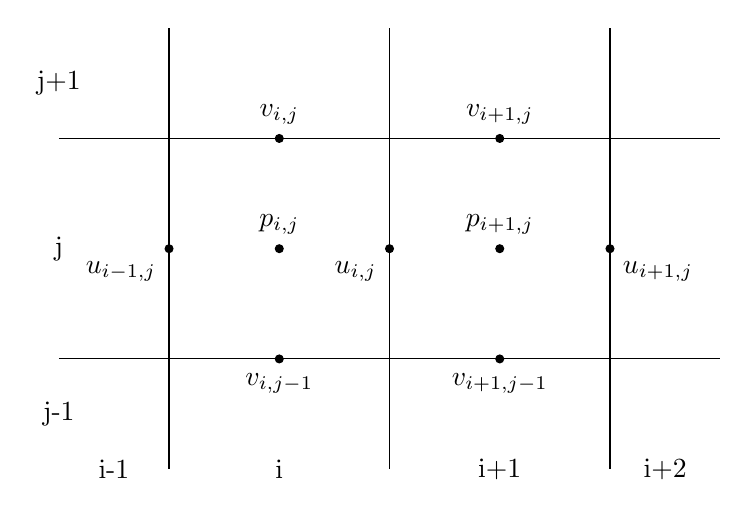
\begin{tikzpicture}[scale=1.4]

\draw (0, 1) -- (6, 1);
\draw (0, 3) -- (6, 3);

\draw (1,4) -- (1,0);
\draw (3,4) -- (3,0);
\draw (5,4) -- (5,0);

\node at (0, 0.5) {j-1}; 
\node at (0, 2) {j}; 
\node at (0, 3.5) {j+1};

\node at (0.5, 0) {i-1}; 
\node at (2, 0) {i}; 
\node at (4, 0) {i+1};
\node at (5.5, 0) {i+2};

\node[label=above:{$p_{i,j}$}, draw, circle, fill, minimum size=0.1cm, inner sep=0pt] at (2, 2) {};
\node[label=above:{$p_{i+1,j}$}, draw, circle, fill, minimum size=0.1cm, inner sep=0pt] at (4, 2) {};

\node[label=below left:{$u_{i-1,j}$}, draw, circle, fill, minimum size=0.1cm, inner sep=0pt] at (1, 2) {};
\node[label=below left:{$u_{i,j}$}, draw, circle, fill, minimum size=0.1cm, inner sep=0pt] at (3, 2) {};
\node[label=below right:{$u_{i+1,j}$}, draw, circle, fill, minimum size=0.1cm, inner sep=0pt] at (5, 2) {};

\node[label=above:{$v_{i,j}$}, draw, circle, fill, minimum size=0.1cm, inner sep=0pt] at (2, 3) {};
\node[label=above:{$v_{i+1,j}$}, draw, circle, fill, minimum size=0.1cm, inner sep=0pt] at (4, 3) {};

\node[label=below:{$v_{i,j-1}$}, draw, circle, fill, minimum size=0.1cm, inner sep=0pt] at (2, 1) {};
\node[label=below:{$v_{i+1,j-1}$}, draw, circle, fill, minimum size=0.1cm, inner sep=0pt] at (4, 1) {};

\end{tikzpicture}
    \caption{Discretization points for each variable on the staggered grid\cite{book:griebel1998numerical}}
    \label{fig:staggered_grid}
\end{figure}

Each of the variables is located at a different position on the grid cell.
Horizontal velocity $u_{i,j}$ is at the midpoint of the right cell edge, vertical velocity $v_{i,j}$ is at the midpoint of the top cell edge, and pressure $p_{i,j}$ is at the midpoint of the cell.
% Staggering the variables in this manner avoids oscillation in the pressure value caused by odd-even decoupling.
This is used to solve odd-even decoupling\cite{Harlow1965NumericalSurface}: for a fluid at rest (i.e. $u = v = 0$) the continuous solution is that the pressure $p$ is a constant across the grid.
However were this to be discretized using central differences with all variables in the same locations, it would also be possible for a checkerboard of pressure values to form, and for oscillation to take place\cite{book:griebel1998numerical}.
This is prevented by staggering the variables.
\cite{peric1988comparison} shows that this is also preventable through colocated grids, where a single grid is used for all variables and the velocities of each side of the cell are found using interpolation.
These cell sides are implicitly staggered relative to the pressure and so avoid this problem.

To allow for derivatives to be accurately calculated for cells on the edges of the grid, boundary cells are added around each grid.%\todomark{figure}
The cells on the edges of any obstacles in the simulation are also marked as boundary squares.
For a finite domain of size $(imax, jmax)$ this leads to a final grid size of $(imax + 2)$ by $(jmax + 2)$, where valid fluid values fall in the ranges %
%$1 \leq i \leq imax$, $1 \leq j \leq jmax$
$i \in \{1..imax\}$, $j \in \{1..jmax\}$.

The physical dimensions of each grid space are represented by \deltaX{}, \deltaY{}.
This allows the derivatives of $u$ and $v$ to be calculated by finding the centered differences.
\begin{align}
    \left[\frac{\partial{u}}{\partial{x}}\right]_{i,j} := \frac{u_{i,j}-u_{i-1,j}}{\delta{x}}, 
    & \quad %
    \left[\frac{\partial{v}}{\partial{y}}\right]_{i,j} := \frac{v_{i,j}-v_{i,j-1}}{\delta{y}}
\end{align}
% TODO multicolumn
% \begin{multicols}{2}
%   \begin{equation}
%     a=b
%   \end{equation}\break
%   \begin{equation}
%     b=c
%   \end{equation}
% \end{multicols}
The partial derivatives for pressure $\partial{p}/\partial{x}, \partial{p}/\partial{y}$ are found in the same way.
The remaining derivatives, including second derivatives and $\partial{uv}/\partial{x}, \partial{uv}/\partial{y}$, can also be discretized by taking the difference across midpoints of their respective dimensions\cite{hirt1976}.
%

\subsection{Timestep Calculation}
\label{sec:TimestepCalculation}
Each simulation tick simulates a discrete amount of time known as a timestep \deltaT{}.
This timestep is not a fixed value, and typically one would want to select as large a timestep as possible.
However, there are constraints on it's maximum value which depend on the simulation state.

As the derivatives are calculated between adjacent grid points, it is impossible to accurately simulate a timestep where fluid moves between non-adjacent grid cells \todopending{Figure?}.
%[Peyret&Taylor,1983]or[Roache,1976].Anadaptivestepsizecontrolbasedonthesestabilityconditionsis usedin[Tome&McKee,1994].
% The simulation cannot accurately solve a timestep in which particles move completely over a cell (see Figure \todocite{}).
To prevent this the timestep \deltaT{} is calculated from the fluid velocities to make it impossible.
\begin{equation}
    \delta{t} = \tau * \text{min}\left(
        \frac{Re}{2}\left(
            \frac{1}{\delta{x}^2} + \frac{1}{\delta{y}^2}
        \right)^{-1},
        \frac{\delta{x}}{|u_{max}|},
        \frac{\delta{y}}{|v_{max}|}
    \right)
\end{equation}

Because the new velocities calculated in this tick may be larger than $u_{max}$ and $v_{max}$, the safety factor $\tau \in [0, 1]$ is used to ensure the timestep is large enough to account for it\cite{TOME1994171}.

\subsection{Tentative Velocity}
The final values of $u$ and $v$ are defined as
\begin{equation}
\begin{aligned}
    u^{(n+1)} &= u^{(n)} + \delta{t}
    \left[
        \frac{1}{Re}
        \paren{\partialderiv{^2u}{x^2} + \partialderiv{^2u}{y^2}} - \partialderiv{(u^2)}{x} - \partialderiv{(uv)}{y} + g_x - \partialderiv{p}{x}
    \right] \\
    v^{(n+1)} &= v^{(n)} + \delta{t}
    \left[
        \frac{1}{Re}
        \paren{\partialderiv{^2v}{x^2} + \partialderiv{^2v}{y^2}} - \partialderiv{(uv)}{x} - \partialderiv{(v^2)}{y} + g_y - \partialderiv{p}{y}
    \right]
\end{aligned}
\end{equation}
However, as these depend on the partial derivatives of $p$, which itself depends on velocity, they cannot be solved analytically.
In order to iteratively find $p$ the variables $f$ and $g$, for horizontal and vertical ``tentative velocity'', are introduced.
\begin{equation}
\begin{aligned}
    f^{(n)} := u^{(n)} + \delta{t}
    \left[
        \frac{1}{Re}
        \paren{\partialderiv{^2u}{x^2} + \partialderiv{^2u}{y^2}} - \partialderiv{(u^2)}{x} - \partialderiv{(uv)}{y} + g_x
    \right] \\
    g^{(n)} := v^{(n)} + \delta{t}
    \left[
        \frac{1}{Re}
        \paren{\partialderiv{^2v}{x^2} + \partialderiv{^2v}{y^2}} - \partialderiv{(uv)}{x} - \partialderiv{(v^2)}{y} + g_y
    \right]
\end{aligned}
\end{equation}
\begin{equation}
\begin{aligned}
    u^{(n+1)} = f^{(n)} - \delta{t}\frac{\partial{p^{(n+1)}}}{\partial{x}} \\
    v^{(n+1)} = g^{(n)} - \delta{t}\frac{\partial{p^{(n+1)}}}{\partial{y}}
    \label{eq:uv_modified}
\end{aligned}
\end{equation}

\subsection{Solving the Poisson Equation with SOR}
\label{sec:SimulationPoisson}
% Two phases - calculating the RHS, then solving
For continuity to be achieved, the final velocity values must fulfil the continuity equation (\cref{eq:NavierStokesContinuity}), the time discretization of which is shown below:
\begin{equation}
    \frac{\partial{u^{(n+1)}}}{\partial{x}} + \frac{\partial{v^{(n+1)}}}{\partial{y}} = 0
\end{equation}
This means that the total amount of fluid entering a cell in tick $n+1$ is equal to the amount of fluid leaving, which must be the case otherwise the amount of fluid per cell wouldn't be constant and the fluid would be compressed.

Substituting the formulae in \cref{eq:uv_modified} into this relation and rearranging gives
\begin{equation}
    \frac{\partial^2{p^{(n+1)}}}{\partial{x^2}} + \frac{\partial^2{p^{(n+1)}}}{\partial{y^2}} = \frac{1}{\delta{t}}\left(\frac{\partial{f^{(n)}_{i,j}}}{\partial{x}} + \frac{\partial{g^{(n)}_{i,j}}}{\partial{y}}\right)
\end{equation}
The right hand side of this equation is constant for timestep $n$, so can be precalculated and assigned to its own variable $rhs$.
\begin{equation}
rhs_{i,j} := \frac{1}{\delta{t}}\left(\frac{\partial{f^{(n)}_{i,j}}}{\partial{x}} + \frac{\partial{g^{(n)}_{i,j}}}{\partial{y}}\right)
\end{equation}
\begin{equation}
\frac{\partial^2{p^{(n+1)}}}{\partial{x^2}} + \frac{\partial^2{p^{(n+1)}}}{\partial{y^2}} = rhs_{i,j}
\end{equation}
Discretizing this gives
\newcommand{\discretized}[4]{#1^{#2}_{#3,#4}}
\newcommand{\pdisc}[3]{\discretized{p}{(#1)}{#2}{#3}}
\newcommand{\fdisc}[3]{\discretized{f}{(#1)}{#2}{#3}}
\newcommand{\gdisc}[3]{\discretized{g}{(#1)}{#2}{#3}}
\newcommand{\ebounds}[1]{\discretized{\epsilon}{#1}{i}{j}}
\begin{multline}
    \frac{\pdisc{n+1}{i+1}{j} - 2\pdisc{n+1}{i}{j} + \pdisc{n+1}{i-1}{j}}
    {(\delta{x})^2} + 
    \frac{\pdisc{n+1}{i}{j+1} - 2\pdisc{n+1}{i}{j} + \pdisc{n+1}{i}{j-1}}
    {(\delta{y})^2}
    % = \frac{1}{\delta{t}}\paren{
    %     \frac{\fdisc{n}{i}{j} - \fdisc{n}{i-1}{j}}{\delta{x}} + 
    %     \frac{\gdisc{n}{i}{j} - \gdisc{n}{i}{j-1}}{\delta{y}}
    % }
    = rhs_{i,j}
\end{multline}
and taking the simplest boundary conditions\cite{book:griebel1998numerical}
\begin{align}
    p_{0,j} &= p_{1,j}, & p_{i_{max+1},j} &= p_{i_{max},j} & j \in \{1..j_{max}\} \\
    p_{i,0} &= p_{i,1}, & p_{i,j_{max+1}} &= p_{i,j_{max}} & i \in \{1..i_{max}\} \\
    f_{0,j} &= u_{0,j}, & f_{i_{max},j} &= u_{i_{max},j} & j \in \{1..j_{max}\} \\
    g_{i,0} &= v_{i,0}, & g_{i,j_{max}} &= v_{i,j_{max}} & i \in \{1..i_{max}\}
\end{align}
resolves the equation to:
\begin{multline}
    \frac{\ebounds{E}(\pdisc{n+1}{i+1}{j} - \pdisc{n+1}{i}{j}) - \ebounds{W}(\pdisc{n+1}{i}{j} - \pdisc{n+1}{i-1}{j})}
    {(\delta{x})^2} \\
    + \frac{\ebounds{N}(\pdisc{n+1}{i}{j+1} - \pdisc{n+1}{i}{j}) - \ebounds{S}(\pdisc{n+1}{i}{j} - \pdisc{n+1}{i}{j-1})}
    {(\delta{y})^2}\\
    % = \frac{1}{\delta{t}}\paren{
    %     \frac{\fdisc{n}{i}{j} - \fdisc{n}{i-1}{j}}{\delta{x}} + 
    %     \frac{\gdisc{n}{i}{j} - \gdisc{n}{i}{j-1}}{\delta{y}}
    % }
    = rhs_{i,j}
    \label{eq:poisson_pre_sor}
\end{multline}
where $\epsilon_{i,j}^{\{N,S,E,W\}}$ represents the boundary squares (shown here for North, but it extends to the other directions)
\begin{equation}
    \epsilon_{i,j}^{N} = \begin{cases}
        0 & \text{The square directly above $i,j$ is a boundary}\\
        1 & \text{The square directly above $i,j$ is \emph{not} a boundary}
   \end{cases}
\end{equation}


\begin{figure}[t]
\centering
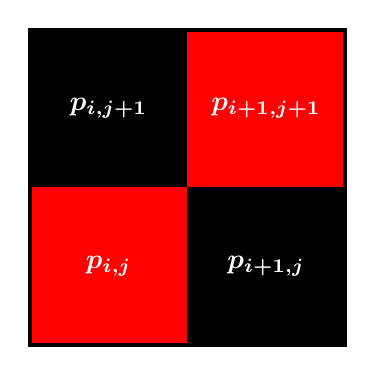
\begin{tikzpicture}[scale=1]
\draw[ultra thick, fill=red] (0,0) rectangle (4,-4);
    \foreach \row in {0,1} {
        \foreach \column in {0} {
    \fill ({4*\column + mod(\row,2)*2}, -\row*2) rectangle +(2,-2);
        }
    }
% \matrix (m) at (0,0) [matrix of nodes,nodes={},
%   anchor=north west,column sep={2cm,between origins},
%   row sep={2cm,between origins}] {
%  {\color{white}{$p_{i,j+1}$}} & {$p_{i+1,j+1}$} \\
%  {$p_{i,j}$} & {\color{white}{$p_{i+1,j}$}} \\
% };
\node at (1,-1) {\color{white}{$\bm{p_{i,j+1}}$}};
\node at (1,-3) {\color{white}{$\bm{p_{i,j}}$}};
\node at (3,-1) {\color{white}{$\bm{p_{i+1,j+1}}$}};
\node at (3,-3) {\color{white}{$\bm{p_{i+1,j}}$}};

% \matrix[matrix of nodes,nodes={draw}]{A & B & C & D & E\\f & G & H & I & J};
\end{tikzpicture}
    \caption{Example checkerboard pattern used for red/black splitting}
    \label{fig:redblack_checkerboard}
\end{figure}
Over the whole grid, this results in a linear system of equations over the inputs $p_{i,j} \forall i \in \{1..i_{max}\}, j \in \{1..j_{max}\}$.
These can be decoupled by partitioning $p$ into red and black squares by a checkerboard pattern (see \cref{fig:redblack_checkerboard}).
As each individual cell only depends on the adjacent values, iterations of Successive Over-Relaxation (SOR) can be performed on red and black in turn to reach a final value\footnote{This could equally be done without partitioning $p$, but the partitioning splits the SOR into separate phases which can then be parallelized. Normal SOR cannot be parallelized\cite{Adams1982AMS}.}\cite{young1971iterative}:
\begin{equation}
    \beta_{i,j} := \frac{\omega}{\left(\frac{\epsilon_{i,j}^E+\epsilon_{i,j}^W}{(\delta{x})^2} + \frac{\epsilon_{i,j}^N+\epsilon_{i,j}^S}{(\delta{y})^2}\right)}
    \label{eq:poisson_beta}
\end{equation}
\begin{multline}
    p^{it+1}_{i,j} := (1 - \omega)p^{it}_{i,j} + \\
    \beta_{i,j} * \left(
    \frac{\epsilon_{i,j}^E p^{it}_{i+1,j}+\epsilon_{i,j}^W p^{it}_{i-1,j}}{(\delta{x})^2} + 
    \frac{\epsilon_{i,j}^N p^{it}_{i,j+1}+\epsilon_{i,j}^W p^{it}_{i,j-1}}{(\delta{y})^2} -
    rhs_{i,j}
    \right)
    \label{eq:poisson_final}
\end{multline}

These iterations are continued until the L2 norm\cite{l2norm} of the residuals (the difference between the left-hand side as calculated and the expected right-hand side of \cref{eq:poisson_final} for each cell) falls below a specific tolerance\footnote{In the ACA coursework this tolerance was relative to the L2 norm of $p$, although this was not directly specified by the book.}\cite{book:griebel1998numerical}.

\subsection{Final Velocity Calculations}
% Update Velocity, applyBoundaryConditions
Once the final values of $p$ have been calculated the velocity values $u,v$ can be found with \cref{eq:uv_modified}.
The boundary conditions for velocity must then be applied.
There are four relevant types of boundary condition\footnote{The book specifies five, including a Periodic Boundary Condition, which the ACA system does not support.}, which are applied depending on the type of boundary.
\begin{enumerate}
    \item No-Slip condition - no fluid penetrates the boundary, and fluid does not move past it i.e. the boundary applies friction.
    \item Free-Slip condition - fluid may not penetrate the boundary, but no friction is applied. Only tangential velocity is preserved for adjacent fluids.
    \item Inflow - fluid is flowing in constantly, so the velocity is set to a constant value. 
    \item Outflow - velocity perpendicular to the surface is preserved and fluids may flow out.
\end{enumerate}
\todopending{Might need equations here?}

% \subsection{Overall Simulation Pipeline}
\todopending{Pipeline figure? Might be better to leave it to full report...}

\section{Optimization}
\label{sec:Research:Optimization}
Optimizing simulations is important in all cases, even those that are not real-time, as it allows the engineers using the software to iterate faster on their designs.
When the extra constraint of real-time speeds is added, it becomes even more important.
This research is mostly complete, although more can be done if the simulation needs to get even faster.

\subsection{Background}
One of the first papers on optimizing a CFD simulation was released in 1995\cite{paper:1995CfdOpt:1383209}.
This paper considered the effect of automatic compiler parallelization and optimization of a full CFD program, and the steps a programmer must take to guide the compiler i.e. avoiding false sharing.
The program was only executed on the CPU, as General Purpose GPU computing (GPGPU) had not yet taken hold.

GPGPU was first used for CFD simulations in 2004 with this paper\cite{paper:2004CfdGPU:10.1109/SC.2004.26}.
This used the ``fragment shading'' stage of the GPU rendering pipeline to perform the computation, as standalone ``compute'' pipelines were only exposed by APIs from 2007 onwards.
Such APIs include CUDA (2007)\cite{tool:CUDAProgrammingV1}, OpenCL (2008)\cite{tool:OpenCL1.0PressRelease}, DirectX's DirectCompute (2009)\cite{tool:DirectComputePresentation}, and OpenGL 4's compute shaders (2012)\cite{tool:OpenGLComputeShaderExt}.
% TODO - OpenGL compute extensions may have existed before this.

Since 2007, using GPGPU for CFD has become a large topic of study, as investigated in detail by \cite{paper:GPGPUSummary:10.1007/s11227-013-1015-7}.
While the concept of accelerating a fluid simulation on the GPU is not new, much of the novelty of our optimizations will stem from the interaction between the simulation and the other systems at work.
As an example, if the simulation were to be modifiable with user input, introducing this new data and updating the boundary conditions in an efficient manner becomes a new problem.
\subsection{Previous Work}
\label{research:prev_work}
As work on CFD progressed some optimizations were developed that change the simulation pipeline and provide an overall speedup.
Some of these were adapted into my ACA coursework submission\cite{modules:aca257submission}, which this project is based on, and carry over into the CUDA version.


Given the definition of $\beta$ in \cref{eq:poisson_beta}, the value of $\beta_{i,j}$ does not change over the course of the simulation and so can be precalculated before the simulation starts.
Additionally if it can be guaranteed that for every boundary square $p = 0$, which can be done either by never updating their pressure values or by updating them with $\beta_{i,j} = 0$, then $\epsilon_{i,j}$ doesn't need to be evaluated during the simulation at all.
These optimizations increased the runtime speed of the Poisson evaluation by 2.24x\footnote{The $\beta$ precalculation increased speed by 1.4x, and the removal of $\epsilon$ increased speed by 1.6x.\cite{modules:aca257submission}}, and they have been kept in the CUDA program.

The book states an alternate solution where $\epsilon$ is set to 1 at all times and pressure values on boundaries are copied from adjacent fluid squares\cite{book:griebel1998numerical}.
This apparently stops noncontinuous starting velocities from producing nonphysical pressure values.
\label{ext:PressureValues}

% 1 on red/black
% The example implementation and the ACA implementation both use Red-Black Successive Over-Relaxation (SOR).
% Red-black SOR was first used to solve a system of linear equations on vector and parallel computersystems by Adams and Ortega [1], although introduced earlier (e.g., by Young [119]). Liu et al. [65] provideda more detailed analysis of red-black SOR implemented on GPUs
% NOTE - the Liu et al. there is a pretty close project

% In this method, the grid is split into red and black squares with a checkerboard pattern\todomark{figure}.
% First the values at red squares are updated, which depend only on the black squares.
% Then, the black squares are updated, which depend only on the red squares.
As stated in \cref{sec:SimulationPoisson}, red/black SOR is used to iteratively solve the Poisson equation.
% The red and black operations can be performed in parallel, but in both the ACA coursework and the CUDA program this has not been done\footnote{It has also been marked as a potential extension}.
In the initial ACA coursework the values ($f$, $g$, $p$, $rhs$) for red and black data were stored in the same arrays.
This was problematic as data of the same color was never contiguous, and any iteration looking for just red values would get a cache line with both colors, leading to half of each cache line being wasted.
To fix this, red and black data is split into separate arrays before starting the Poisson solver.
This has been carried over into the CUDA implementation.

% Parallelization i.e. Vectorization, OpenMP?
% "The ACA coursework used OpenMP to provide thread-level parallelization in kernels, which is automatically provided when using a GPU."
The ACA solution used OpenMP\cite{OpenMPHomeOpenMP} to automatically parallelize the Poisson solver (and other program elements) by column.
That is, each thread was given a group of columns to process.
This was not needed in the CUDA version as each GPU kernel is implicitly parallelized over many GPU threads.

The ACA solution included optimizations exploiting properties of the original code, such as floating point precision, to speed up calculations while producing identical results.
These optimizations include using fused multiply-add\cite{Muller2010TheInstruction} in some places (but not all), precalculating divisions with double-precision floats, and skipping the residual calculation phase altogether.
As this project is focused on improving upon the accuracy of the ACA submission, instead of producing bit-identical results, these optimizations have generally not been implemented into the CUDA program.\footnote{The CUDA program still lacks a residual phase, but this is planned to be implemented later.\label{sec:OptimizationReAddingResidual}}

% Paragraph on ACA-specific (FMA tricks, removing divisions, residual removal)
% "Other courseworks specifically tied to the ACA coursework were"...

%% ACA Recap(cite)
%% - Residual removal. (probably needs to be reversed)
%% - beta precalc (check if somewhere/ in book)
%% - mathematical optimization to remove branches (check if in book)
%% - FMA trickery (cite FMA properties)
%% - red/black rearranging (defo mentioned in top level paper, find citation from that)
%% - vectorization AVX/SSE (can most likely cite something here)
%%     - Note that 8-vector was tested,but 4-vector was faster
%% - removing divisions (maybe?)
%% - OpenMP (irrelevant here but can provide a citation? and should be noted because it provides parallelism which is then replaced by the GPU)


% TODO - tick pipeline figure with ACA additions (ex. r/b splitting)

\subsection{Future Work}
\label{sec:FutureOptimization}
Along with the items mentioned in the previous section, there are some optimizations planned to be implemented over the Christmas break and during Term 2.

CUDA devices are split into many threads, which are split into groups of 32 that are executed concurrently as a warp\cite{tool:CUDAProgrammingV1}.
If the threads in a warp attempt to access multiple words in the same cache line, the access is \textit{coalesced}\cite{NVIDIAHowBlog} and only one cache line needs to be fetched for the warp to continue.
Otherwise if the accesses all touch different cache lines, every cache line needs to be fetched before execution can continue for any of the threads.
The CUDA program attempts to arrange the threads such that they coalesce accesses, but it has not been verified to work yet.

% Const Restrict Pointers for __ldg (https://dl.acm.org/doi/pdf/10.1145/3238147.3241533 tries to do this automatically and found a perf boost, can cite that or cite other papers on it).
% \todomark{This seems more like a statement of an optimization than a "Future Work".}
The CUDA C Programming Guide\cite{NVIDIAGlobalGuide} states that read-only memory can be read into a special data cache using the \texttt{\_\_ldg()} intrinsic.
The compiler may insert this automatically when it detects that data must be read-only.
The use of \texttt{const} and \texttt{\_\_restrict\_\_} qualifiers on pointers that are read-only is encouraged to make read-only data obvious.
In \cite{10.1145/3238147.3241533} it was found that introducing these qualifiers where possible led to large speedups in pointer heavy applications, and while our case may not use many pointers this should still be implemented wherever possible.
In the CUDA implementation templates for input and output matrices are used that include these qualifiers automatically, and all kernels are assumed to restrict all pointer arguments.
However it has yet to be verified that \texttt{\_\_ldg()} is inserted in the correct places, which should be done in the future.

% GPU Vectorization (cite).
The ACA solution used Intel AVX and SSE instructions\cite{IntelCorporationIntroductionExtensions} to calculate four Poisson values at once\footnote{Vectors of eight were tried but were found to be slower than four.}.
Each CUDA core of a GPU has access to four-element vectors without any extensions, so this vectorization can be extended per CUDA core. 
This has not been implemented in the CUDA program, but is a future extension to test.
This may or may not actually speed up computation, as the memory bandwidth would be quadrupled and the computation is already excessively parallel.

% Mention parallelization with OpenMP
% did already?

% Highly optimized reductions (cite).
Calculating the simulation timestep and calculating the residual for a Poisson iteration both require a reduction over large blocks of data.
Highly parallel GPU optimizations have already been studied extensively, so it should be trivial to implement a very fast generic reduction kernel.
In \cite{CUDAParallelReduction} seven kernels are described, in ascending order of speed.
Currently the CUDA program uses the second kernel model, and this is planned to be moved up to the seventh kernel in the future.


\section{Visualization}
For the engineers and scientists developing simulations, it is important for a visualization to be completely accurate and show the data in as much detail as possible.
However there are other groups that may not have as deep of an understanding, but whose actions and decisions should still be informed by the simulation results.
Currently the research is focused on learning lessons from the ACA coursework's provided visualization.
For a visualization to cater to these groups well further research in this space is required.

\subsection{Background}
%Earliest found instance of interactive visualizaion is (https://dl.acm.org/doi/10.5555/509740.509745) in 2002. Did not use the GPU for any computation.
One of the earliest CFD interactive visualizations was in 2002, which had a simulation running slower than real time on a separate computer to the real-time visualization\cite{paper:2002vis:10.5555/509740.509745}.
%\todocite{https://dl.acm.org/doi/10.5555/509740.509745}
Decoupling the simulation speed from the visualization speed allowed for high framerates to be achieved for the user interface, however any changes made from the user interface had a delay of 0.5 seconds before being reflected in the simulation.

Many scientific visualizations of fluid flow exist already.
% To name two examples, streak lines are commonly used for visualizing velocities in a still image\todocite{}, and colored smoke is used to visualize airflow on moving objects in videos\todocite{}.
To name two examples, streak lines and fluid colors are used for visualizing fluid flow\cite{video:AutodeskFlowDesign}.
These methods are perfectly fine for those who understand what these elements mean, i.e. what the colors represent, and what the optimal airflow would look like.
However, for those unfamiliar with the simulation these methods can be difficult to understand.

This project aims to develop new visualization techniques for two-dimensional simulations that are more intuitive than the current offerings, that can be extended to three dimensions easily.
Using high-speed rendering APIs like Vulkan\cite{tool:Vulkan} will allow these visualizations to be made even more complex while maintaining high speeds.
Furthermore, our approach may allow for slight inaccuracies to be introduced for the sake of intuitivity, which has not been explored in research to the author's knowledge.

% However novelty in the visualization space not pursued.

% Introduction of Vulkan allows for more efficient rendering, which can be made more complex than before.
\subsection{Previous Work}
The original coursework\cite{modules:CS257Coursework} provided a simple image visualizer for a simulation state, which evaluated one of two quantities over the grid and produced a \texttt{.ppm} image with the result.
These quantities were Vorticity ($\zeta$), the strength of vortical (a.k.a. rotational) motion at each point in the grid; and Stream Function ($\psi$), the contours of which define streamlines.
Streamlines are lines that are parallel to the velocity vector at each point, allowing the long-term flow of particles to be represented with a single line, and thus in a static image.\cite{NASADefinitionStreamlines}
The quantities are defined by \cref{eq:zeta,eq:vorticity}, as specified in \cite{book:griebel1998numerical}.
Examples of these modes are shown in \cref{fig:ppms}.

\begin{equation}
    \zeta(x,y) := \frac{\delta{u}}{\delta{y}} - \frac{\delta{v}}{\delta{x}}
    \label{eq:zeta}
\end{equation}
\begin{equation}
    \frac{\delta{\psi}(x,y)}{\delta{x}} := -v,\quad \frac{\delta{\psi}(x,y)}{\delta{y}} := u
    \label{eq:vorticity}
\end{equation}

\begin{figure}[ht]
    \centering
    \subcaptionbox{Vorticity $\zeta$\label{fig:zeta_ppm}%
    }[\linewidth]{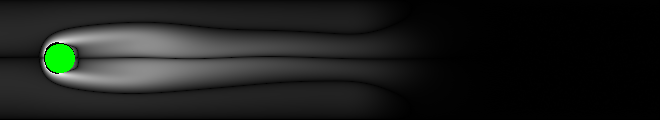
\includegraphics[width=\linewidth,natwidth=660,natheight=120]{Ch20Research/figures/output_zeta.png}
    }
    
    \subcaptionbox{Stream Function $\psi$\label{fig:psi_ppm}%
    }[\linewidth]{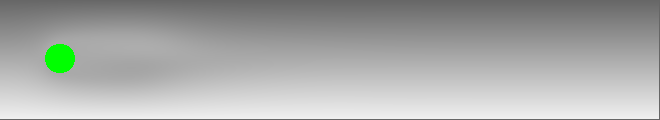
\includegraphics[width=\linewidth,natwidth=660,natheight=120]{Ch20Research/figures/output_psi.png}
    }
    
    \subcaptionbox{Pressure $p$\label{fig:pressure_ppm}%
    }[\linewidth]{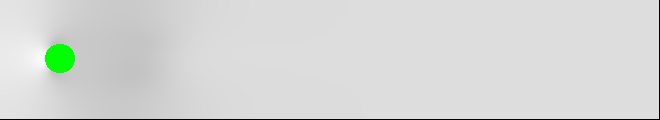
\includegraphics[width=\linewidth,natwidth=660,natheight=120]{Ch20Research/figures/output_pressure.png}
    }
    \caption{Examples of the three outputs available from the original visualization.}%\\These all visualize the output of a modified ACA coursework running for 10 seconds on the provided input data.
    %  all visualizing the same state.
    \label{fig:ppms}
\end{figure}
% Criticism of zeta, psi, pressure implementation
The vorticity image in \cref{fig:zeta_ppm} competently shows which areas of the grid contain particle movement.
However near the edges of the obstacle circle (shown in green) the edges are black, implying no movement or rotation, which is incorrect and also a distracting artifact for the viewer.
These are due to the imprecise nature of the original code, which only uses the differences to the East and South to find $\zeta$.
This breaks down when the squares in these directions are boundaries, and the program defaults to zero.
A better solution would be to take the central difference whenever possible, and to fall back to using only one side when adjacent to an boundaries.
This would mean the only points where this breaks down are where a square is surrounded by boundaries on opposite sides, which is much less likely and would also likely break other areas of the simulation.
% \todomark{This scenario would also break other parts of the sim. maybe mention that.}
% \todomark{Does this need a figure? I don't think it's worth it}

The Stream Function visualization (\cref{fig:psi_ppm}) is nearly impossible to visually parse, which makes sense as the velocity information is encoded in the differences between adjacent squares and not directly in the colors.
The Stream Function is not intended to be directly visualized, but instead used to find streamlines which can be visualized directly.

\label{sec:VizPressureCritique}
During program development a third mode was added which directly visualized the pressure values to aid in debugging, but this was not a very useful visualization as seen in \cref{fig:pressure_ppm}.
Pressure is only ever referenced in the Navier-Stokes equation (and subsequently the algorithm) as a relative value.
However, the simulation in practice ends up increasing all cells by a small amount each iteration.
This overall increase in pressure values is ignored by the simulation, but the visualization doesn't adjust for it.
In this example, the pressure values have all increased so even the lowest pressure value is a mid-gray.
If the program simulated for too long, the pressure values would become too high and the visualization would be entirely white.
This pressure mode has been carried over to the CUDA program as a placeholder visualization, but will be replaced.
\subsection{Future Work}
% Boids(cite), particles(cite), things proposed by the book
While a purely image-based approach to visualizing properties can be useful, other approaches allow for i.e. multidimensional quantities such as velocity to be expressed much more easily.
In the case of velocity, vector fields and particle tracing are both shown in \cite{book:griebel1998numerical} to be effective.

Given that our simulation is realtime, we can also add changes over time to the mix.
Tracing particle paths and rendering them as a line could be replaced by actually watching the particles move over time.
Particle movement could also be enhanced with extra behaviour similar to that of BOIDs\cite{BOIDS_10.1145/37401.37406}, which among other things implement Collision Avoidance.
This would prevent particles from overlapping and getting visually lost.
Vorticity/rotational movement could be visualized by adding particles to the grid that rotate over time based on he vorticity at their location.
This could allow the vorticity to be represented in the same view as the other parts of the simulation, instead of creating a dedicated view separate from velocity/pressure.

% !TEX root =  ../FinalReport.tex

\chapter{Ethical, Social, and Legal Issues}
\label{sec:EthicalSocialLegal} 
As predicted in the Specification and Progress Report, there have been no ethical or social issues with the development of this simulation and visualization.
The simulation has been derived from code provided to the students for the ACA coursework\cite{modules:CS257Coursework}, which itself is directly derived from a book\cite{book:griebel1998numerical} available at the Warwick Library\cite{ethics:WarwickLibraryFluidSimBook}.
The visualization is entirely original code, and the inspirations and research used to design it have all been cited.

% During the development of the visualization, feedback may be gathered as to which elements are most intuitive.
% Any such feedback will be restricted to the opinion of friends and family, and as such comes under the category of ``Student projects with primarily an educational purpose''\cite{UniversityofWarwickEthicalConsent}, so does not require ethical review.
% This feedback would be gathered according to the University guidelines\cite{ethics:WarwickConsent}, and any gathering will follow the Data Protection Act 2018\cite{ethics:DataProtection2018}.

% Mention BCS Code of Conduct, completely pointless but do it lol
To ensure the work can be trusted, and to maintain professional standards, the BCS Code of Conduct\cite{ethics:BCSCodeOfConduct} has been followed.
Professional standards were maintained during development, and research performed has been effectively referenced to a high standard.


% !TEX root =  ../FinalReport.tex

\newcommand{\must}[0]{\textbf{must}}
\newcommand{\should}[0]{\textbf{should}}
\newcommand{\shouldnt}[0]{\textbf{should not}}


\chapter{Project Requirements}
\label{sec:Requirements}
Ahead of initial development, a set of requirements were created to further specify the project goals.
These requirements evolved as more research was completed, for example the visualization-related requirements were only determined after visualization research completed (see \cref{sec:ProjectManagement}).
This chapter shows the functional and non-functional requirements, prioritized as either \must{}-have or \should{}-have.
Complex requirements have sub-requirements, which clarify certain features that must/should be present for the top-level requirement to be met.
%  which  into sub-requirements in some cases to clarify the broad points.
% Each requirement is assigned a 
The hardware and software constraints for the program are also shown.



% These basic functional and non-functional requirements define the baseline the final result will be measured against.
% \todomark{Elaborate on requirements}

% Functional Requirements define the actions a program must/should be able to perform, such as \cref{req:GenerateState} stating ``the system must be able to generate initial simulation states''.
% The functional requirements, the tests performed to check them, and the outcomes have been listed in \cref{tab:functional_req}.

% Non-functional Requirements do not define actions, but rather define properties of those actions that must be met.
% As an example \cref{reqN:SimSpeed} states that with the same initial input, the CUDA simulation ``should run at least 2x as fast as the original coursework''.


\section{Functional Requirements}
Functional Requirements define actions a program must/should be able to perform.
\begin{reqF}
    \item \label{req:StoreState} The system \must{} store simulation state in a file or set of files.
    \item \label{req:LoadState} The system \must{} be able to load the initial state of a simulation from these file(s).
    \item \label{req:GenerateState} The system \must{} be able to generate initial simulation state files.
    \item \label{req:HeadlessSim} The system \must{} be able to simulate from an initial state for a set amount of time without visualizing.
    \begin{reqF}
        \item \label[reqFi]{req:HeadlessOutput} This mode \must{} be able to store the final state to output file(s).
    \end{reqF} 
    \item \label{req:VizSim} The system \must{} be able to simulate from an initial state for an indeterminate amount of time while visualizing.
    \begin{reqF}
        \item \label[reqFi]{req:VizPauseResume} This mode \must{} allow the user to pause and resume the simulation.
        \item \label[reqFi]{req:VizSaveState} This mode \should{} be able to save it's state to output file(s) when requested.
        \item \label[reqFi]{req:VizManip} This mode \should{} allow the user to manipulate the simulation or visualization state while simulating.
        \item \label[reqFi]{req:VizLockedFPS} This mode \should{} be able to run at a locked frame-rate.
        \item \label[reqFi]{req:VizFlatOut} This mode \should{} be able to run as fast as possible, without locking the framerate.
        \item \label[reqFi]{req:VizSomeSpeed} This mode \must{} be able to perform at least one of \cref{req:VizLockedFPS,req:VizFlatOut}.
    \end{reqF} 
    \item \label{req:GPUCapable} Both methods of simulation \must{} be capable of using the GPU for simulating.
    \item \label{req:Compare} The system \must{} be able to compare how similar two simulation states are.
    \begin{reqF}
        \item \label[reqFi]{req:CompareBinary} This comparison \should{} produce a binary SIMILAR/NOT~SIMILAR verdict using heuristics.
    \end{reqF}
    
    \item \label{req:VizLayers} The visualization \must{} consist of multiple layers which can be individually controlled.
    \begin{reqF}
        \item \label[reqFi]{req:VizLayersBackground} The visualization \must{} always display a background layer which shows the simulation obstacles in a different color to the fluid.
        \item \label[reqFi]{req:VizLayersScalar} The visualization \must{} be able to display an optional scalar quantity (e.g. pressure) using a color scale, where the value is within a user-defined range.
        \item \label[reqFi]{req:VizLayersVector} The visualization \must{} be able to display an optional vector quantity (e.g. velocity) using a vector field, where the magnitude is within a user-defined range.
        \item \label[reqFi]{req:VizLayersParticle} The visualization \must{} feature an optional particle simulation, where particles are continuously emitted and move with the velocity of the field.
    \end{reqF}
    \item \label{req:VizAutoRange} The scalar and vector quantities (\cref{req:VizLayersScalar,req:VizLayersVector}) \should{} have an auto-range function to automatically calculate the range based on the values present.
    \item \label{req:VizColors} All colors used in the visualization (e.g. particle colors, the scalar color scale) \should{} be user-controlled.
    \item \label{req:VizParticleEmission} The locations of particle emitters \should{} be user-controllable.
\end{reqF}

\pagebreak
\section{Non-Functional Requirements}
Non-functional Requirements do not define actions, but rather define properties of those actions or the program that must be met.
\begin{reqNF}
    \item \label{reqN:LargeData} The system \must{} be capable of operating on large datasets (e.g. 4096x4096 grids) without failing.
    \item \label{reqN:Resources} The system \must{} be efficient and avoid wasting any resources allotted to it.
    \item \label{reqN:SimilarOutput} The simulation \must{} produce similar results to the original simulation when equivalent initial state is used.
    \item \label{reqN:SimSpeed} The simulation \should{} run at least 2x as fast as the original simulation when equivalent initial state is used.
    \item \label{reqN:Realtime} The visualized simulation \must{} run in real-time at framerates~$\ge$~30 FPS for some outputs.
    \item \label{reqN:VizSpeed} The visualization features \shouldnt{} have a significant impact on the framerate.
    \item \label{reqN:Intuitive} The visualized simulation \should{} intuitively represent the fluid flow such that it can be understood by someone unfamiliar with fluid simulation.
    \item \label{reqN:VizParticleAdvanced} The particle simulation (\cref{req:VizLayersParticle}) \should{} demonstrate advanced behaviour to make the visualization more intuitive e.g. avoiding clumping.
    \item \label{reqN:Documented} The system \must{} be fully documented and maintainable. % TODO Wheeler referenced BCS code of conduct again??
    \item \label{reqN:UsageGuide} The system \should{} have a simple guide to common operations for new users to refer to.
    \item \label{reqN:DCSCompile} The system \should{} be fully compilable and executable from a DCS machine with minimal extra installations.
\end{reqNF}

\section{Hardware and Software Constraints}
\label{sec:Requirements_HardwareSoftware}
As this simulation uses a GPU, the developer must have one available for debugging and testing the program.
As the CUDA API is used to implement the simulation (see \cref{sec:LibrarySelection}), the program requires an NVIDIA GPU to run.
Due to the COVID situation the only hardware used to test the device was the researcher's GTX~1080.

The high-speed rendering requirements of the program necessitated the use of Vulkan over OpenGL.
Vulkan gives the developer more fine control over scheduling, and allows the hardware to take shortcuts that it may not be able to do under OpenGL.
For more on this decision see \cref{sec:LibrarySelection}.
% !TEX root =  ../FinalReport.tex

\chapter{Design}
\label{sec:Design} 

while building a large project it's important to develop a consistent, logical, and properly separated design; both to make initial development easy and to make it intuitive for any future developers to understand.
This applies to all aspects of the program including the codebase (i.e. which classes exist and how they communicate), how the program implement complex processes (such as the simulation/visualization), and how the end user will eventually use the program.

This section first separates the codebase into layers and analyses them in order.%from lowest to highest.%in order from the lowest-level to the highest-level.
% This section first separates the codebase into layers, then analyses these layers in order from the lowest-level to the highest-level.
All notable design decisions for each layer are noted, and the means of interaction between these layers are documented.
The final section, for the Command-Line layer, also documents the design of the command-line interface and the file formats used to store simulation states.


\section{Code Structure}
\begin{figure}
    \centering
    \makebox[\textwidth][c]{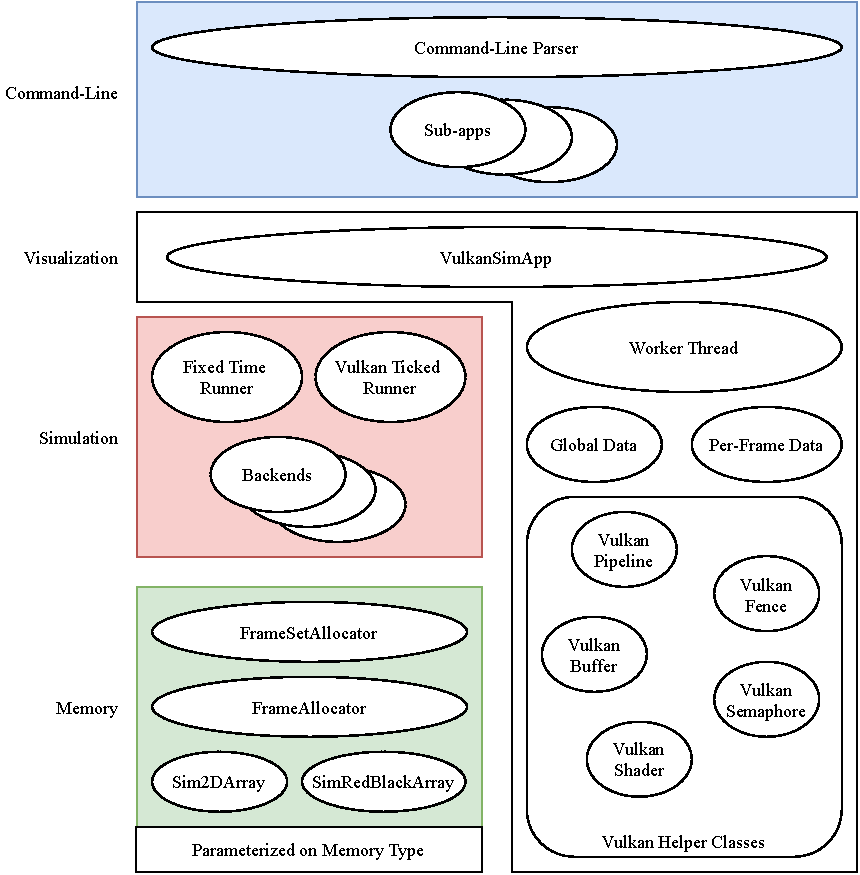
\includegraphics[width=1\linewidth]{Ch42Design/figures/FinalReport_DesignStructure.pdf}}
    \caption{Overall Code Structure}
    \label{fig:designstructure}
\end{figure}
% The overall structure of the project is shown in \cref{fig:designstructure}.
The project structure, shown in \cref{fig:designstructure}, is split into four layers: Command-Line, Visualization, Simulation, and Memory.
Each element broadly represents a C++ class which depends on the classes defined below it.

The Command-Line layer has a Command-Line Parser, which converts the passed-in argument strings to usable representations, and a set of sub-apps.
Each sub-app implements one of the subcommands shown in \cref{sec:DesignSubcommands}.
The figure shows all classes relevant to the \shell{run} subcommand, which shows a visualized simulation.

The Visualization layer contains a high-level \code{VulkanSimApp} class, which initiates all visualization-related code.
Beneath that the Worker Thread handles most Vulkan API calls, and depends on multiple sets of data built with Vulkan helper classes.
This layer uses classes from the Simulation layer, which are reused for the \shell{fixedtime} subcommand to avoid code duplication.

The Simulation layer consists of two main elements: the Runners, and the Backends.
The Runners use different strategies for invoking a Backend - the \code{FixedTimeRunner} runs the simulation flat out until a specific time is reached and outputs the final state, and the \code{VulkanTickedRunner} runs the simulation for small timesteps while synchronising with other Vulkan elements.
Each Backend implements the same interface, so Runner implementations can be Backend-agnostic.
The \code{FixedTimeRunner} supports all of the defined Backends (see \cref{sec:DesignBackends}), but the \code{VulkanTickedRunner} can only use the Vulkan-compatible CUDA backend.

Finally, the Memory layer exposes APIs for the Backends to allocate simulation memory.
Runners decide how many `frames' to create (see \cref{sec:DesignSimNBuffer}), and use the \code{FrameSetAllocator} to create a set of \code{FrameAllocator}s.
The Backends use each \code{FrameAllocator} to allocate a set of buffers, which are then used to store simulation data.
These buffers are represented with \code{Sim2DArray} and \code{SimRedBlackArray} instances.
The \code{SimRedBlackArray} splits a given grid size into two halves, one storing entirely red elements and one storing entirely black elements, and can be configured to store an additional full matrix (helpful for e.g. pressure, where both representations are useful.)

All elements of the Memory layer are parameterized on the type of memory.
This can be CPU memory allocated with \code{malloc} and \code{free}, CUDA Unified Memory (see \cref{sec:Design:Simulation}), or Vulkan on-device memory. 
The memory type affects not just the allocation method, but also the properties it has e.g. CPU memory cannot be accessed from the GPU.
Using parameterized array classes allows these differences to be expressed while keeping a consistent interface.

\section{Simulation \& Memory Layer}
% The simulation component of the program is used in both the headless and real-time modes, so the design needs to be suitable for working with both.

% \subsection{Backends}
To allow easy comparisons between CPU and GPU simulations the program contains multiple simulation backends.
%which can be requested when running a headless simulation\footnote{The realtime visualization currently only supports the CUDA-based backend, violating \cref{req:GPUCapable}.}.
The headless and visualized simulations use a \texttt{--backend} command line option to allow the user to choose the backend from this selection:\label{sec:DesignBackends}
\begin{itemize}
    \item Null, a backend which does no simulation for testing purposes.
    \item CPU Simple, equivalent to pre-optimization ACA code.
    \item CPU Optimized, equivalent to the submission for ACA, bit-equivalent to CPU Simple.
    \item CPU Optimized Adapted, a version of CPU Optimized slightly modified to be closer to the GPU version.
    \item CUDA Backend V1, the only GPU-based backend.
\end{itemize}

The only modification present in the CPU Optimized Adapted backend is the removal of double-precision floating point logic, which is not present on the GPU for speed concerns.
It still isn't identical to the CUDA environment, as CUDA aggressively contracts floating point operations to fused multiply-add while the CPU compiler does not.
The other CPU optimizations are present on the GPU where possible: the residual check between each Poisson phase is still removed, and the red-black data is still separated into separate arrays. 
% However once the GPU introduces residual checking for the iterative solver, or any other major changes to the pipeline, they will be introduced into this backend to ensure a like-for-like comparison.

% Each backend implements a consistent interface (\todoref{UML Figure for interface}), allowing the implementations of the headless and visualized running modes to be backend-agnostic.
% The headless simulation mode can use all of the available backends.
% The visualization only supports the CUDA backend, as it is the only backend which is compatible with Vulkan.
% While the code for the visualized running mode could theoretically use any Vulkan-compatible backend, the CUDA backend is the only Vulkan-compatible backend present in the final program.

\subsection{CUDA Design}\label{sec:Design:Simulation}

The CUDA backend implements each stage of the simulation (\cref{fig:SimStages}) as one or more CUDA Kernels.
Each CUDA Kernel represents a computation for a single grid cell, which is executed by a GPU thread.
The grid is split into small `blocks' of threads, and the threads within each block are executed by a Streaming Multiprocessor (SM) in groups of 32 (a `warp').% in parallel over the entire grid.
% These threads are split into a hierarchy as described in \todocite{https://www.nvidia.com/content/PDF/fermi_white_papers/NVIDIA_Fermi_Compute_Architecture_Whitepaper.pdf}.
% ``A GPU executes one or more kernel grids; a streaming multiprocessor (SM) executes one or more thread blocks; and CUDA cores and other execution units in the SM execute threads.''
The grids and blocks can be specified in 1D, 2D, or 3D depending on the dimensionality of the problem.
Our program uses a 2D grid for most kernels, because each computation reads adjacent data in 2D space.
Reduction kernels treat the 2D grid as a flat 1D array, because there is no need for adjacent data.

The CUDA backend must execute both with Vulkan (when visualized) and without Vulkan (when headless).
This affects the type of memory used in the simulation.
When visualized, crucial data such as velocity and pressure are stored in shared Vulkan-CUDA memory, to allow direct usage from both APIs without copying the data.
In all other cases CUDA Unified Memory is used, which can be paged between the CPU and GPU on-demand without manually mapping it across\cite{Harris2017UnifiedBlog}.
This allowed for granular debugging during development, as GPU kernels could be easily swapped out for known-correct CPU implementations without having to move memory manually.

% \todomark{CUDA Unified memory allows for granular debugging by combining known-correct CPU implementations with GPU kernels} 

\subsection{N-Buffering}\label{sec:DesignSimNBuffer}
When developing the Visualization, it was noted that keeping a separate copy of the simulation output would allow the visualization to run in parallel with the simulation, without the simulation overwriting data currently being visualized.
To allow this, N-buffering was introduced to the simulation backends and to aspects of the visualization.
Multiple `frames' are stored, where each one contains all data used in a simulation tick.
Each simulation tick is assigned to a specific frame chosen by the Runner, and only the data in this frame is written to.
The index of the last-written frame is tracked, and is used as the input for the next simulation tick.
During a simulation of frame \#N, the contents of the other frames is constant and can be read out without any race conditions.

% \subsection{Design Optimizations}
% The residual check after every Poisson phase is still removed, although it was planned to be 

\pagebreak
\section{Visualization Layer}
This section details the code implemented in order to efficiently and effectively visualize simulation results in real time.
This is not related to the \texttt{renderppm} subcommand, which uses CPU code to render a single simulation state as an image.

\subsection{Components}
There are four major components of the visualization which work together to create the final output.
\begin{itemize}
    \item CPU 0 - The Main Thread, which handles the CUDA simulation.
    \item CPU 1 - The Worker Thread, which records and enqueues Vulkan commands.
    \item The GPU, which executes both the CUDA and Vulkan commands.
    \item The Swapchain, which provides render targets that are displayed in the application window.
\end{itemize}
The GPU itself has three phases of execution, performed sequentially for each frame (\cref{tab:gpuexecution}).
Each frame accesses a set of per-frame data, which is reused in a circular buffer.
Each phase for the frame will use this data.
\begin{table}[h]
    \centering
    \begin{tabular}{l|c}
    Name & Abbreviation \\
    \hline
    Simulation & Sim \\
    Visualization Compute (e.g. simulating particles) & VizComp \\
    Visualization Graphics & VizGfx \\
    \end{tabular}
    \caption{GPU Execution Phases, with abbreviations}
    \label{tab:gpuexecution}
\end{table}

A key design goal with the visualization was to maximize GPU utilization.
The CPU work is much less complicated than the GPU work, so the CPU should always be able to keep the GPU fed with new work.
If the CPU failed to do this, the GPU would waste time idling when it could be doing useful work.

\begin{figurepage}
\begin{figure}[p]
    \centering
    \makebox[\textwidth][c]{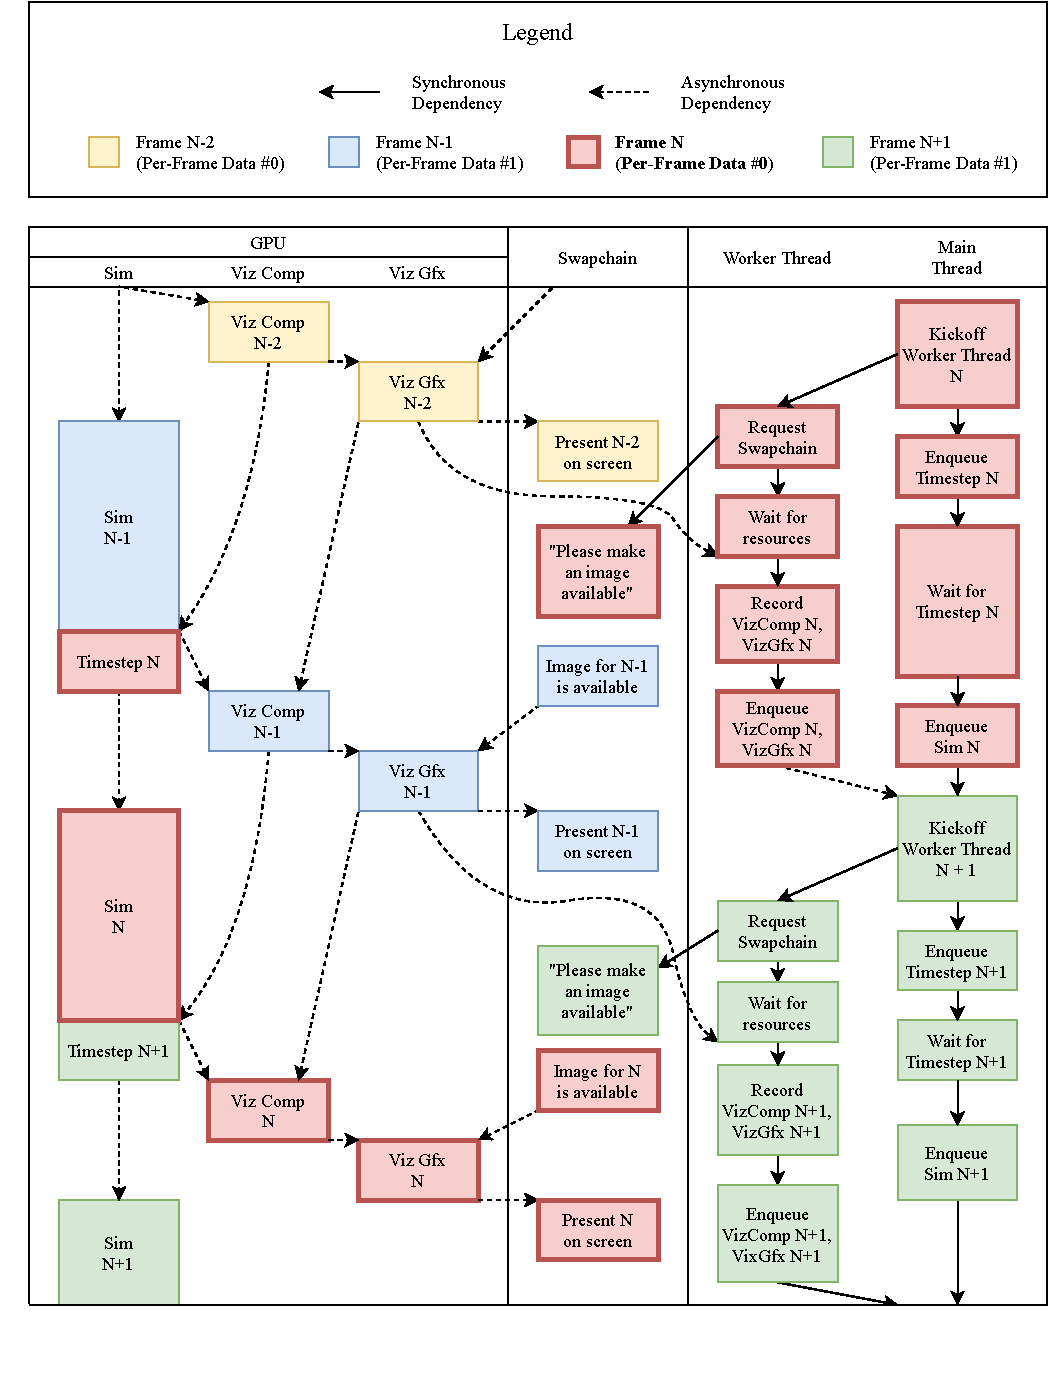
\includegraphics[width=1.1\linewidth]{Ch42Design/figures/FinalReport_Timing.pdf}}
    \caption{Timing Breakdown of four visualization frames, assuming two sets of per-frame data.}
    \label{fig:DesignTiming}
\end{figure}
\end{figurepage}

\subsection{Timing Breakdown}\label{sec:Design:Viz:Timing}

\cref{fig:DesignTiming} shows a breakdown of multiple frames of simulation and visualization, focusing on \textbf{frame \#N} which is highlighted in red.
It includes both synchronous and asynchronous dependencies.
A task with synchronous dependencies starts immediately once all dependencies finish.
A task with asynchronous dependencies can only start once all dependencies are finished, but may not start until later.

The main thread begins by initiating the worker thread before handling the simulation.
Before any CUDA work is enqueued, a semaphore is used to create a dependency on a previous compute job (`Viz Compute $N - 2$'). % Semaphore computeFinishedCanSim.
This compute cycle and the incoming CUDA work will access the same per-frame data\footnote{Viz Gfx jobs don't access the raw simulation buffers, so it doesn't delay the simulation.}, so this dependency prevents the simulation from writing to the data while the compute job reads from it.
For higher efficiency this dependency could be inserted on `Sim $N$' instead, but in practice it would not affect the results.

The VulkanTickedRunner enqueues CUDA work to determine the maximum timestep for the next tick (`Timestep $N$' in the diagram), waiting to get the results back on the CPU, and enqueueing the rest of the simulation based on the calculated timestep (`Sim $N$')\footnote{`Sim' and `Timestep' work are enqueued on the same CUDA stream, so they are implicitly ordered.}.%\todocite{CUDA stream ordered}
If visualization requested a larger timestep than the calculated maximum, the process would be repeated until the total requested timestep had elapsed.
Once `Sim $N$' is finished, it signals a semaphore to allow `Viz Comp $N$' to continue the frame. % Semaphore simFinishedCanCompute

The worker thread asks the swapchain for an image using the \texttt{vkAcquireNextImageKHR} function.
This returns an index which will eventually become available, and a semaphore which will be signalled once this happens.
Before `Viz Gfx $N$' can render to this image, it has to wait for this semaphore to signal it is ready. % Semaphore imageAcquiredCanRender
The thread then waits for frame $N-2$ to finish using the Vulkan resources in Resource Set 0, before it uses them to record `Viz Comp $N$' and `Viz Gfx $N$'. % Fence frameCmdBuffersInUse
The Viz jobs have some semaphores to guarantee ordering:
`Viz Gfx $N$' must start after `Viz Comp $N$' finishes, which must start after `Sim $N$' finishes. % Semaphore simFinishedCanCompute, computeFinishedCanRender
`Viz Comp $N$' also has to wait for `Viz Gfx $N - 1$' to finish to avoid race conditions - all `Viz Comp' and `Viz Gfx' jobs share global memory instead of per-frame memory to avoid data copying. % Semaphore renderFinishedNextFrameCanCompute
Once `Viz Gfx $N$' finishes, it signals a semaphore to tell the swapchain/OS to present the newly rendered frame to the screen.
The worker thread records and enqueues the above work for the GPU.
Once the worker thread has finished it signals the main thread, and once the main thread finishes enqeueing `Sim $N$' the process restarts.

It's worth noting that based on these dependencies some GPU work could theoretically run in parallel, such as `Viz Comp $N$' and `Timestep $N-1$'.
Unfortunately in practice this doesn't happen.
Running parallel compute workloads was introduced in the Ampere GPU generation \cite{nvidiaAmpereWhitepaper}, such as the RTX~3000 series, and is not supported on the researcher's GTX~1080.
This also affects the work breakdown, preventing smaller pieces of work (such as computations for separate visualization layers) from running in parallel.
In the future this could be mitigated by using an Ampere-level GPU, or by running the simulation and visualization on separate GPUs.

\subsubsection{Synchronization}
In order to implement an unlocked framerate without running the simulation faster than real-time, the time between frame `starts'\footnote{i.e. kicking off the worker thread} is measured to determine how long an average simulation frame takes. 
% The desired `simulations-per-second' is set by the user, and 
The program predicts how long a simulation frame \emph{would} take, and combines that with the requested simulation rate\footnote{e.g. 120 simulation ticks per second} to predict if the next frame should be a simulation frame.

When running with an unlocked simulation rate, the average time per simulation frame is chosen as the timestep for the next simulation tick.
This is capped with sensible minimum/maximum limits to avoid instability from performance outliers.

\subsection{Visualization Work Breakdown}\label{sec:Design:Viz:Breakdown}
As specified in the Requirements (\cref{sec:Requirements}) the selected visualization layers are the Background, Quantity-by-Scalar, Quantity-by-Vector, and Particle Simulation.
The Background and Quantity-by-Scalar layers are visualized at the same time for simplicity.
Accounting for this, the breakdown of required work for each layer is shown in \cref{fig:VizBreakdown}.

\begin{figure}
    \centering
    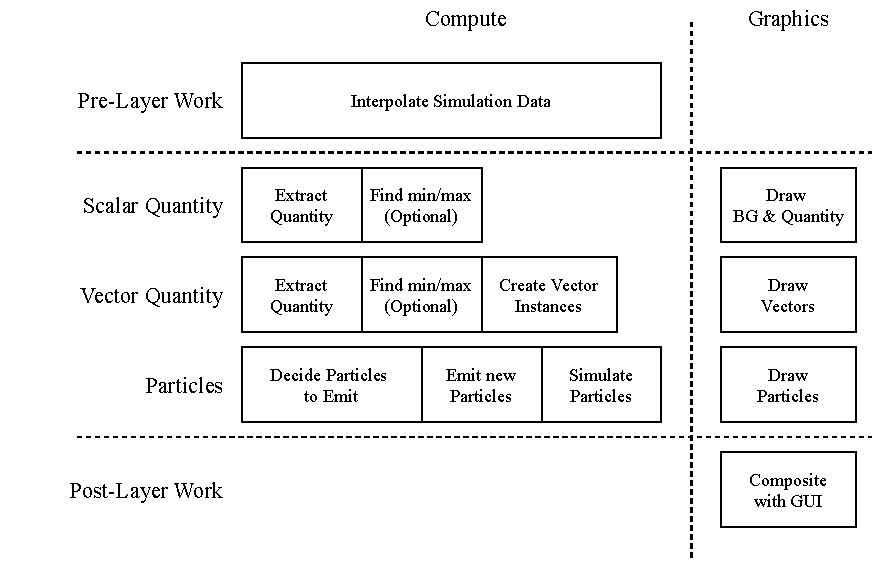
\includegraphics[width=\linewidth]{Ch42Design/figures/FinalReport_VizWork.pdf}
    \caption{Visualization Work Breakdown}
    \label{fig:VizBreakdown}
\end{figure}

The Compute sections are implemented using Vulkan Compute Shaders\cite{TheKhronosGroupVulkanSpec}, which are nearly equivalent to CUDA Kernels and are invoked similarly.
The Graphics sections are implemented using Vertex and Fragment Shaders, where the Vertex Shader determines the onscreen positions of the vertices that make up a model, and the Fragment Shader determines the color of the onscreen pixels between those vertices.

\subsubsection{Data Interpolation}
The simulation stores data on a staggered grid (\cref{fig:staggered_grid}), but this is not amenable for some visualization tasks.
The first step of the visualization is to move the exposed simulation data into a 2x resolution texture, applying interpolation where necessary, allowing the GPU to sample the exposed data at arbitrary points using the texture filtering hardware.
This applies trilinear interpolation, as required for the particle simulation.

\subsubsection{Auto-ranging}
Both Quantity-by-Scalar and Quantity-by-Vector have an optional auto-range mode, where the minimum and maximum values for the quantity are calculated and used instead of the user-defined quantity scale.
This requires a GPU reduction, which is implemented in Vulkan just like it is in CUDA, using the second kernel of \cite{CUDAParallelReduction}.
In order to easily render the data in both cases the selected quantity is extracted to two buffers using a specialized compute shader.
The first buffer includes the quantity with a `fluidmask' which shows if the selected pixel is a fluid or obstacle, and is used for the rendering.
The second buffer has a min/max property for each element, and is used as the input to the reduction.

\subsubsection{Indirect Instanced Rendering}
For Quantity-by-Vector and the Particle Simulation, the final outputs are rendered using Instanced Rendering.%\todocite{Instanced Rnedering}
The same model is rendered $N$ times, and the Vertex Shader gets an `instance index' $0 \le i < N$.
This index is used to look-up the instance's position/orientation in a separate buffer.
This method is much faster than rendering each instance separately, as it requires fewer draw calls on the CPU.
\begin{figure}
    \centering
    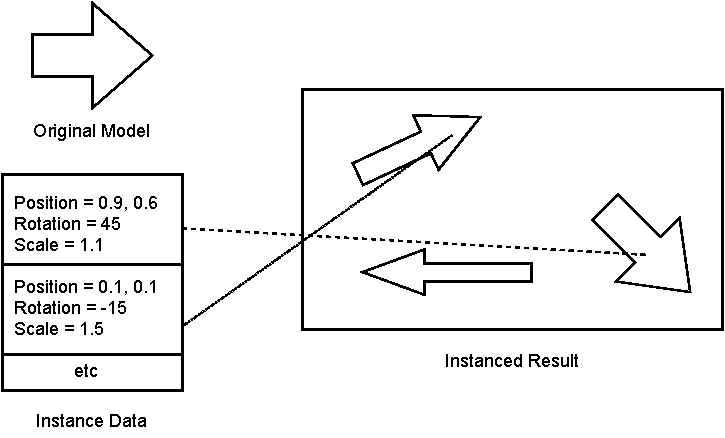
\includegraphics{Ch42Design/figures/FinalReport_InstancedRendering.pdf}
    \caption{Instanced Rendering Demonstration}
    \label{fig:InstancedRendering}
\end{figure}

When recording the command buffer on the CPU, the number of instances for both layers is not yet known.
For Quantity-by-Vector the number of vectors is dependent on the simulation output, because vectors cannot be placed on obstacles.
Some Particles may be killed by the previous round of simulation, so they cannot be predicted either.
To mitigate this, Indirect invocations are used for the vector/particle rendering and the particle simulation.
Instead of specifying the instance count at record time, a reference to a GPU buffer is used.
This GPU buffer contains the required parameters for the instanced rendering/compute dispatch, and can be atomically written by the GPU in a separate compute shader.

Creating new vectors/particle instances is done safely on the GPU using growable lists and atomic variables.
Each growable list consists of an array of values with a maximum length, and a `current size' variable.
When a value is added, the `current size' variable is incremented atomically, and the pre-increment value is then used to index the array and write the new instance parameter.
When a value is removed, the `current size' variable is decremented atomically, and the post-increment value can be used to see the deleted value.
Within a compute shader invocation, a list can only be growable or shrinkable but cannot be both.
Despite this limitation the lists are suitable to implement the technique from \cite{WickedEngineParticles}.

\subsubsection{Final Composite}
As a final step the visualization output is rendered with the other GUI elements.
This step is controlled by the Dear ImGUI library, not my own code (see \cref{sec:LibrarySelection}).
An example of the visualization GUI is shown in \cref{fig:viz_gui}.

\begin{figure}[b]
    \centering
    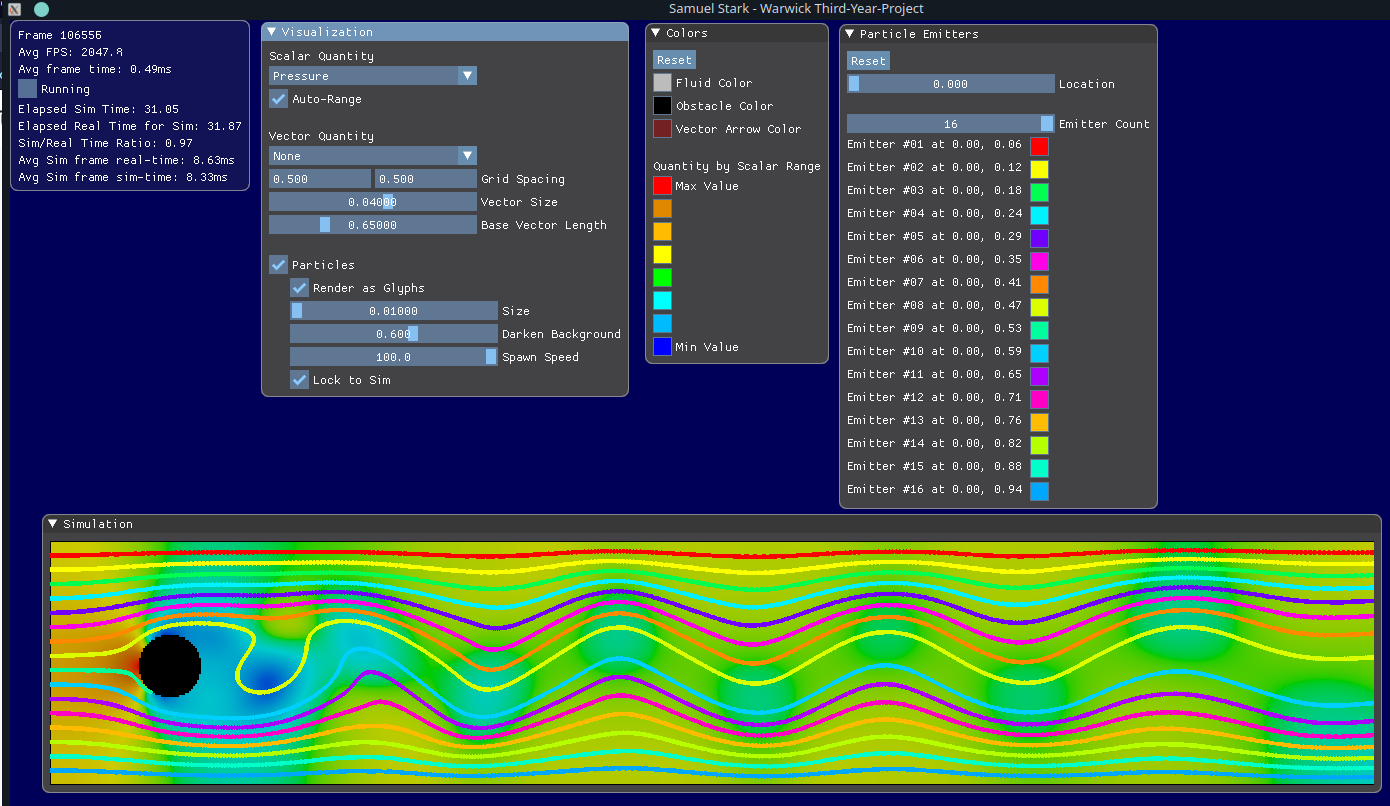
\includegraphics[width=\linewidth]{Ch42Design/figures/dan.png}
    \caption{Example of the Visualization GUI}
    \label{fig:viz_gui}
\end{figure}


\section{Command-Line Layer \& Program Usage}
% \todomark{intro para?}

% \subsection{Command-Line Interface}
The compiled binary uses a command-line interface to configure and run one of many subcommands available.
These subcommands are:\label{sec:DesignSubcommands}
\begin{itemize}
    \item \texttt{makeinput}, which generates simulation input files, fulfilling \cref{req:GenerateState}.
    \item \texttt{fixedtime}, which runs a headless simulation for a fixed time, fulfilling \cref{req:HeadlessSim}.
    \item \texttt{compare}, which compares two simulation states for equality (see \cref{sec:Comparisons}), fulfilling \cref{req:Compare}.
    \item \texttt{renderppm}, which visualizes a static simulation state using the techniques from \cref{sec:Research:Viz:ACA}.
    % \item \texttt{convert2newbinary}, for converting ACA simulation state files to a potential new format (see \cref{sec:FileFormat}). Currently a no-op.
    \item \texttt{run}, which starts a real-time visualized simulation, fulfilling \cref{req:VizSim}.
\end{itemize}
Splitting the program into subcommands was inspired by Git\cite{tool:Git}, and avoids creating separate binaries for each operation.
Each subcommand can be configured with command-line options conforming to POSIX standard\cite{IEEE2018UtilityConventions}.
Examples of using the program are in \cref{fig:BashExampleUsage}.
\input{Ch42Design/figures/usage_example}

\subsection{Generating Inputs}
The \texttt{makeinput} subcommand allows input simulation states to be generated from image files.
Each pixel of the input image represents a cell of the grid, including padding cells\footnote{This can allow the padding cells to be fluids rather than boundaries, which is incorrect. In the future this will be changed to add padding cells once the image is parsed.}, where non-black pixels are denoted as boundary cells and are fluid cells otherwise.
The example in \cref{fig:ExampleMakeinput} shows an example file which creates a rectangular obstacle, and the visualization of the generated state.
\input{Ch42Design/figures/example_makeinput}

Velocities and pressure in every cell are interpolated horizontally - \SI{1}{m/s} east at the left edge, \SI{0}{m/s} at the right.
This alleviates simulation instability near obstacle edges, an advantage over having a constant initial velocity across the field.
% For velocities, this is \SI{1}{m/s} east, equal to the default flow of incoming fluid, which may cause issues with correctness.
One such instability would be a situation where fluid is occluded from the input direction by an obstacle, but moves east anyway with no reason to do so.
%it would not be correct for that fluid to move) 
% This will likely be changed to zero out initial velocity, requiring some simulation to take place before the fluid begins to move.

The exact initial value of pressure is inconsequential as the simulation only cares about the difference between cells.
The pressure is set to 0 at all points, representing a constant pressure across the simulation grid.
This is inconsistent with the nonzero velocities mentioned above, but applying variable pressure made the system more unstable.

\subsection{File Formats}\label{sec:FileFormat}
To fulfil \cref{req:StoreState} two file formats have been defined to store simulation data and parameters.

\subsubsection{Fluid Parameters}
Parameters that are characteristic of a particular fluid or simulation type are stored in a ``Fluid Parameters'' file.
This includes the Reynolds number, the timestep safety factor, and the maximum iteration count for the Poisson solver.
They are stored in a JSON format to be human-readable, are reusable for different simulation states, and can be easily edited by the end user.
An example is shown in \cref{fig:FluidParamsExample}.

\input{Ch42Design/figures/example_fluidparams}

\subsubsection{Simulation State}
Data unique to an individual state such as simulation resolution, physical size, and velocity fields are stored in a binary format reused from the original simulation.
As the data is much more sensitive to individual modifications\footnote{i.e. changing a single value in the velocity field can introduce discontinuities}, it makes more sense to store this data in a binary format where it cannot be easily modified by a user.
Additionally, the binary format is much smaller than any text-based format, which helps as the volume of data stored is much larger than that stored in the fluid parameters.

The header consists of a pair of unsigned 32-bit integers specifying the resolution of the simulation, and a pair of 32-bit floating-point numbers specifying the physical dimensions of the simulation.
From there, four sets of data for each column are stored, including the boundary padding squares:
\begin{enumerate}
    \item Horizontal Velocity $u$ (\code{float32})
    \item Vertical Velocity $v$ (\code{float32})
    \item Pressure $p$ (\code{float32})
    \item Cell Flags, defining which adjacent squares are boundaries (\code{uint8})
\end{enumerate}
This structure is somewhat unintuitive and error-prone, an example being the Cell Flags which may end up being inconsistent between adjacent cells, but it has been kept for the sake of compatibility with the original simulation.


\subsection{Comparison Heuristics}\label{sec:Comparisons}
In the \shell{compare} subcommand heuristics are used to judge if one simulation is accurate and precise with respect to the other.
This does not quite fulfil \cref{req:CompareBinary}, as there are two results and two heuristics used instead of just one, but it is useful for comparisons regardless so was not changed.

This assumes one of the supplied states is a known-valid simulation state, and the other is not.
The velocity and pressure values $u, v, p$ of the two simulation states are compared separately.
% The simulation states must be of the same resolution, and should use the same boundary squares (although this is not checked).
The simulation states must be of the same size and use the same obstacle squares.

The comparison is performed by calculating the mean and standard deviation of the square error between the datasets.
These are then compared to tolerance values to produce two binary outputs: ACCURATE if the mean is below tolerance, and PRECISE if the standard deviation is below tolerance.
Examples are shown in \cref{fig:example_comparisons}.

The tolerance for the mean was derived from an expected error magnitude of $\pm 10^{-7}$, which was squared to produce $10^{-14}$.
It is assumed that the standard deviation should always be smaller than the mean, so the tolerance for standard deviation is also $10^{-14}$.
% \todopending{More examination of this? Square error always >0 => if std.dev > mean then distribution cannot be normal? Prob wait for full report}

\input{Ch42Design/figures/example_comparisons}

% % \todomark{UI}


% !TEX root =  ../FinalReport.tex

\chapter{Implementation}
\label{sec:Implementation}

Building the program was a huge technical challenge on many levels, resulting in 8.5k lines of code spread over 146 files in three different programming languages.
% involving three programming languages, % resulting in 8.5k lines of code built with three programming languages 
Solving the more complicated problems required some interesting tricks which may have interacted with lesser-known language features, memory models, and in one case the particulars of the C++17 specification.
The correctness of the resulting program was then ensured through the use of other features, including C++ macros and files that crossed language boundaries\footnote{See \cref{sec:Impl:Viz:CPUGPUSafety}.}.
This chapter documents these tricks and the background needed to understand them.

The first section contains an overview of relevant C++ features, and some other concepts employed while developing the program.
The next section focuses on Code Safety, detecting any faults during compilation and then ensuring any other faults do not then manifest into problematic errors.
As in the Design section, each layer of the codebase is then examined and all interesting problems solved during development are documented.

\section{Preliminary Work \& Background}
The primary languages used in the program are C++17 and CUDA.
This section will explain key elements of C++17 used in the program, the build system, and the external libraries used.

\subsection{C++ Primer}
Virtual classes use virtual functions to allow subclasses to override behaviour in the parent.
The seminal example is creating a parent class \texttt{Animal} which can \texttt{talk()}, and a subclass \texttt{Dog} which overrides \texttt{talk()} to bark. \todomark{Better example/code?}
When a virtual function is called on an object, instead of statically determining which function to call at compile-time, the \emph{vtable} of the object is read out at run-time with the correct function pointer.
In Java and Python all functions are considered virtual, but in C++ virtual behaviour can be selectively enabled.
As each virtual function call requires multiple indirections (object $\rightarrow$ vtable $\rightarrow$ function), the performance is slightly worse than using normal functions.
Virtual functions are avoided where possible in the codebase.
\todomark{Demo code https://godbolt.org/z/jYonzK76r}
\todocite{https://pabloariasal.github.io/2017/06/10/understanding-virtual-tables/}

C++'s largest innovation over C is the template system.
Classes and functions can be `templated' on types or values, and then `instantiated' when these parameters are known.
When such a class or function is instantiated a complete copy is created with the new parameter values, which is compiled and optimized separately from any other instantiations.
This is useful for encoding extra information in a type for safety, e.g. \mintinline{cpp}{VulkanShader<Vertex>} cannot be passed to a function expecting \mintinline{cpp}{VulkanShader<Compute>} because they're independent types.
It's also useful for static function dispatch, as instead of taking a virtual class with a \texttt{talk()} function you can instead template a function on the type of animal it uses, and call the function directly.
This technique is used in the Simulation to efficiently use Backends.
\todomark{https://godbolt.org/z/zz7jvTW6E template vfunc example}

\subsubsection{``Typeclasses''}
In other languages, like Haskell, a typeclass defines some behaviour a class should fit. From \todocite{Learn you a haskell}: ``If a type is a part of a typeclass, that means that it supports and implements the behavior the typeclass describes''.
C++17 does not have a convenient way of denoting this but it is especially helpful when building generic code with templates, as it allows the generic code to make assumptions about what behaviour types will support.
The rest of this chapter will define typeclasses where convenient to describe behaviour shared by certain classes.

\subsection{Build System}
The build system is implemented in CMake as specified in \cref{sec:ProjManagementTools}. %\cite{tool:Cmake}
This section highlights a few changes that were made to an otherwise standard setup to accommodate the project.

\subsubsection{CUDA-less Binaries}
The project can be built to produce both CUDA and CUDA-less binaries, in case it needs to be run on CUDA-less computers.
The list of regular C++ source files and CUDA source files are maintained separately. A CUDA-less binary (\shell{sim\_nocuda}) will only build the C++ files while a CUDA binary (\shell{sim\_cuda}) will build both.
When building the \shell{sim\_cuda} target the preprocessor macro \code{CUDA\_ENABLED} is defined throughout all source files, including the C++ files.
This allows support for CUDA backends in C++ code (i.e. as selectable options on the command-line) to be conditionally enabled without maintaining two copies of the relevant source files.
In \cref{fig:ConditionalCUDA} (which has been amended for brevity), the switch statement only contains a case for CUDA if the directive is set, triggering a fatal error otherwise.
\input{Ch48Implementation/figures/conditional_cuda}


% \todomark{Move Shader Build Infrastructure somewhere else?}
\subsubsection{Shader Build Infrastructure} % Fits in with the build system vibe
The shaders used for visualization are written in GLSL, with appropriate extensions to be compatible with Vulkan.
They are separated by file type, with Vertex shaders in \shell{.vert} files and Fragment shaders in \shell{.frag} files.
As Vulkan does not natively support GLSL, they must be compiled to SPIR-V before they can be used.
CMake does not support GLSL as a first-class language, so a custom build command was used to compile them with \shell{glslc}\cite{GoogleLLCShaderc} when they change.
This allows them to be treated just like any other source file from the programmer's perspective.
The SPIR-V files are placed in a \shell{shaders} directory next to the binaries, where they can be easily accessed and passed to Vulkan.

% \todomark{Code Safety - emphasis on using templates, compile-time checks, and failing that runtime assertions.}

\subsection{Library Selection}
\label{sec:LibrarySelection}
\input{Ch48Implementation/figures/compat_matrix}
CUDA and Vulkan have been chosen as backends, but other backends were also considered.
As the simulation would have to run on DCS systems (\cref{reqN:DCSCompile}) and thus run on Linux, the only possible GPU rendering backends were OpenGL and Vulkan.
However, there were still multiple choices of compute backend:
\begin{itemize}
    \item OpenCL\cite{tool:OpenCL1.0PressRelease} is an ``Open Standard for Parallel Programming of Heterogeneous Systems''\cite{TheKhronosGroupOpenCLInc}.
    \item CUDA\cite{tool:CUDA} is a closed-source library for running parallel code on NVIDIA GPUs.
    \item OpenGL has Compute Shaders\cite{tool:OpenGLComputeShaderExt} which can execute computations outside of the graphics pipeline.
    \item Vulkan also has Compute capability\cite{TheKhronosGroupVulkanGuide}, similar in function to OpenGL.
\end{itemize}
To decide on the compute backend to use, an interoperability matrix was drawn (\cref{fig:LibraryChoices}) to show which libraries could share data without copying it between buffers.
As the researcher was already experienced with Vulkan, and the more granular control it provides would be beneficial to performance, Vulkan was selected as the rendering backend.
This prevented OpenCL and OpenGL from being used as compute backends, as they are not compatible with Vulkan.
CUDA and Vulkan have comparable ability, but CUDA was chosen as the compute backend.
The Vulkan compute shaders are still a very graphics-oriented view of computation, and CUDA would give the researcher experience with other kinds of libraries.
A Vulkan compute backend is used for the visualization portion of the code.

% Not for now, but note that the C++ vulkan bindings are nice. They do end up wrapped in other classes, but they remove the need to remember boilerplate as much.

In other cases, there were clear choices: the SDL2\cite{SimpleHomepage} window and input library and the Dear ImGUI\cite{CornutDearImGui} UI library were chosen due to personal experience.
The \shell{stb\_image.h} header was found to be a simple method of importing image colour data as byte arrays, used for the input generator (\cref{req:GenerateState}).

There are a great many options for Command-Line parsing libraries, even more so because C++ is used instead of C.
A recent survey of the possibilities\cite{attractivechaos2018AC/C++} was whittled down to five options.

\code{getopt}\cite{FreeSoftwareFoundationGetopt3:Page}, \code{argp}\cite{GNUProjectArgpLibrary}, and \code{gopt}\cite{VajzovicGoptLibrary} are C libraries that use arrays of structures to define the required arguments.
Of them, only \code{argp} can automatically generate a \shell{--help} argument, which is a very valuable feature.
\code{cxxopts}\cite{jarro2783Cxxopts:Parser} was considered as a C++ alternative but used very odd syntax for defining arguments.
Ultimately CLI11\cite{CLIUtilsCLI11} was chosen as a modern C++11 library that had native support for subcommands, which were used heavily for separating program components (see \cref{sec:DesignSubcommands}).

% \todomark{Resource Management}

\section{Code Safety}\label{sec:Impl:CodeSafety}
No program is faultless, and when faults manifest during execution it's important to ensure they have a minimal effect on their surroundings.
This program includes many means of detecting errors both at compile-time and run-time to ensure its dependability.

The G++ flag \shell{-Wall} enables many warnings that are emitted at compile-time if potential errors are detected.
Unlike some other languages (i.e. Verilog) these warnings are generally reliable and it is feasible to build a C++ program that compiles without any warnings.
To ensure this the \shell{-Werror} flag is added to upgrade these warnings to compilation errors, ensuring a program which compiles will be warning-free\footnote{Some warnings, such as those from \shell{-Wextra} and those relating to unused variables and parameters, are usually benign so weren't upgraded.}.

Runtime errors are detected with a set of C++ macros that check if required conditions are met.
As there is no liveness requirement for the program, failure triggers an immediate program exit to avoid errors propagating through the system.
The \code{DASSERT} family of macros are included only in Debug builds, and the \code{FATAL\_ERROR} family of macros test both in Release and Debug.
Both families print a message including the file and line of code that triggered the error, and any other relevant debug information.
These families are also integrated with the \code{CHECKED\_CUDA} and \code{CHECKED\_VULKAN} macro families, which surround CUDA/Vulkan function calls and check the returned error codes.
An example is shown in \cref{fig:ImplAssertions}.
\begin{figure}[t]
    \centering
    \begin{subfigure}{0.49\textwidth}
        \begin{minted}{cpp}
if (value == unexpected) {
    FATAL_ERROR(
        "Unexpected Value %d\n",
        value
    );
}
// equivalent to
FATAL_ERROR_IF(
    value == unexpected,
    ...
);
// or
FATAL_ERROR_UNLESS(
    value != unexpected,
    ...
);

// Same, but only fails in Debug builds
DASSERT(value != unexpected);
        \end{minted}
        \caption{Example of assertion macros}
    \end{subfigure}%
    \begin{subfigure}{0.49\textwidth}
        \begin{minted}{cpp}
cudaError_t error = cudaDeviceSynchronize();
FATAL_ERROR_IF(error != cudaSuccess);
// Equivalent to
CHECKED_CUDA(cudaDeviceSynchronize());

auto result = vkDeviceWaitIdle();
FATAL_ERROR_IF(result != vk::Result::eSuccess);
// Equivalent to
CHECKED_VULKAN(vkDeviceWaitIdle());
        \end{minted}
        \caption{Example of API failure safety macros}
    \end{subfigure}
    \caption{Examples of error safety via macros}
    \label{fig:ImplAssertions}
\end{figure}

The final tool for error detection is the Vulkan Validation Layer.
This is a standard Vulkan extension which checks each Vulkan call to ensure the Vulkan specification \cite{TheKhronosGroupVulkanSpec} isn't violated.
These checks are very in-depth, and are a must-have when debugging visualization errors.
The base Vulkan functions don't do this error checking for efficiency's sake, and the program disables these layers in Release mode for the same reason.

\subsection{Smart Resource Classes}
All memory allocations, CUDA objects, and Vulkan objects follow the same allocate/release pattern.
They are not destroyed automatically when they go out of scope, but must be released manually.
This is an error-prone process, as a programmer may forget which resources need to be released or try to release a resource twice.

\begin{figure}
    \centering
    \begin{cppcode}
// Manual handling
{
    auto* semaphore = new Semaphore();
    // do things with semaphore...
    delete semaphore;
}

// Automatic handling
{
    std::unique_ptr<Semaphore> semaphore = std::make_unique<Semaphore>();
    // do things with semaphore...
    // automatically deleted
}
    \end{cppcode}
    \caption{Example of memory management with C++ standard classes}
    \label{fig:ImplUniquePtr}
\end{figure}

Smart resource classes alleviate this by tying the resource lifetime to a C++ object, using the object \emph{destructor} to release the resource.
The prime example of this is \code{std::unique_ptr<T>}, which holds a \code{T*} object and \code{free()}-s it when the object leaves scope (\cref{fig:ImplUniquePtr}).
However this does not easily map to other deletion methods, and the pointer adds an unwanted extra level of indirection.
\code{vulkan.hpp}, included in the Vulkan SDK, includes similar classes for each type of Vulkan resource, but still requires a lot of boilerplate to initially create objects\footnote{Vulkan objects require a full CreateInfo struct to create, rather than taking function arguments.}.
In some cases, it's also more convenient to store multiple resources together, such as a buffer and the device memory it uses, which cannot be directly achieved with either method.
To solve these problems custom smart resource classes are implemented for individual resources and aggregates, with more convenient constructors (see \cref{sec:appx_resourceclasses}).

These smart classes are affected by C++ copy/move semantics.
C++ allows objects to be copied with a copy-constructor, or moved with a move-constructor.
The resource objects should not be copyable as it would become unclear which copy would be responsible for destroying the resource.
The copy-constructor can be deleted to prevent this, but the move-constructor is useful for transferring ownership e.g. from a resource factory to the person using the resource.

When an object is moved, the original version should forget the data it's holding and give it to the new object.
C++ can generate this constructor automatically, but this ``default move-constructor'' will just copy the data across if the data is \textit{TriviallyCopyable}\cite{cpprefMoveConstructor}.
%, and is true for pointers and all CUDA handles.
All pointers and CUDA handles are \textit{TriviallyCopyable}, so they don't get forgotten automatically.
Manually writing each move-constructor to address this would be error-prone, so instead the \code{ForgetOnMove<T>} class is used to wrap these values and automatically forget them when the move-constructor is invoked.
% To avoid manually creating move-constructors, which is error-prone, the \code{ForgetOnMove<T>} class wraps these values and automatically forgets them when the move-constructor is invoked.
The final result is shown in \cref{fig:ForgetOnMoveEx}: a clean, easy, and safe method of implementing new smart resource classes.
% Detecting and mitigating these faults and errors is an important part of effective programming, 
\begin{figurepage}
\begin{figure}
    \centering
    \begin{cppcode}
// Doesn't use ForgetOnMove<>
class ComplexWrapper {
    void* memoryPointer;
    
    // Constructor
    ComplexWrapper(size_t memorySize) {
        // Allocate memory
    }
    // Destructor
    ~ComplexWrapper() {
        if (memoryPointer != nullptr) {
            // Free memory
        }
    }
    
    // Copy constructor - deleted
    ComplexWrapper(const ComplexWrapper&) = delete;
    // Move constructor - complicated
    ComplexWrapper(ComplexWrapper&& movedFrom) {
        this->memoryPointer = movedFrom.memoryPointer;
        movedFrom.memoryPointer = nullptr;
    }
};

// Uses ForgetOnMove<>, is simpler
class SimpleWrapper {
    ForgetOnMove<void*> memoryPointer;
    
    // Constructor as before
    SimpleWrapper(size_t memorySize) {
        // Allocate memory
    }
    // Destructor as before, but checks if the memoryPointer is present
    ~SimpleWrapper() {
        if (memoryPointer.has_value()) {
            // Free memory
        }
    }
    
    // Copy constructor - deleted
    SimpleWrapper(const SimpleWrapper&) = delete;
    // Move constructor - defaulted!
    // We don't have to write this in full
    SimpleWrapper(SimpleWrapper&&) = default;
};
    \end{cppcode}
    % \caption{Example of \code{ForgetOnMove<T>} vs. manual handling.}
    % \caption{Comparing \code{ForgetOnMove<T>} to manual handling.}
    \caption{Automatic forgetting with \code{ForgetOnMove<T>} vs. manual handling}
    \label{fig:ForgetOnMoveEx}
\end{figure}
\end{figurepage}

\pagebreak
\section{Memory Layer}
As mentioned in the Design section, all elements of the Memory system are parameterized on the memory type.
This was accomplished by creating an enum \code{MType} and a set of classes templated on it (\cref{fig:TypeclassMemory}).
These templates were then specialized for each type of memory, implementing the logic for each type separately.
Separate implementations were required due to the unique constraints and allocation methods of each memory type.

\begin{figure}
    \centering
\begin{minted}{cpp}
enum MType {
    CPU,
    Cuda,
    VulkanCuda
};

enum RedBlackStorage {
    RedBlackOnly, // Just store the red and black matrices
    WithJoined // Store the red, black, and combined matrices
};

typeclass DataArray {
    // Has a static value MemType telling you what memory type it takes
    static MType MemType;
    // Has a function for calculating the total bytes used for a matrix
    static size_t sizeBytesOf(Size<uint32_t> size);
}

typeclass FrameAllocator<MType> {
    // Function for allocating a 2D array
    Sim2DArray<T, MType> allocate2D(Size);
    
    // Function for allocating a red/black array
    SimRedBlackArray<T, MType, RedBlackStorage> allocateRedBlack(Size);
}

typeclass FrameSetAllocator<MType, TFrame> {
    std::vector<TFrame> frames;
}
\end{minted}
    \caption{Memory Layer Typeclasses}
    \label{fig:TypeclassMemory}
\end{figure}

\subsection{Array Handles}
The \code{Sim2DArray<T, MType>} and \code{SimRedBlackArray<T, MType, RedBlackStorage>} classes represent handles to 2D arrays of values of type \code{T}.
They implement a common \emph{DataArray} typeclass (\cref{fig:TypeclassMemory}).
They do not own the data they point to, so if a \code{Sim2DArray} is destroyed the referenced memory isn't freed.
Freeing memory is handled by the \code{FrameAllocator} instead.

\code{SimRedBlackArray} serves as an aggregate of \code{Sim2DArray}s, without defining any special behaviour.
It does not specialize on the memory type, but provides two storage variants \code{RedBlackOnly} and \code{WithJoined} (\cref{fig:TypeclassMemory}).

\code{Sim2DArray} implements a set of functions for accessing data from the CPU, CUDA, and Vulkan.%GPU, and as Vulkan handles.
These functions are only present if that access type is supported, so trying to use an unsupported function results in a compile-time error.
Other more generic operations are also supported such as zeroing out memory, copying memory in from different sources, and copying memory out to the CPU.
Each of these is implemented differently based on the memory type, and may not be implemented if the operation is impossible.
For example attempting to `prefetch', i.e. move CUDA Unified Memory to the GPU, is only supported for CUDA Unified Memory and not the other types.
% \todomark{Matrix of supported operations}

\subsection{\texttt{FrameAllocator}}
\code{FrameAllocator<MType>} is an allocator associated with a single memory frame.
The behaviour is specialized for each memory type, but each specialization fits a typeclass (\cref{fig:TypeclassMemory}) for allocating 2D and red-black arrays.
The \code{FrameAllocator} owns these allocations, and when it is destroyed the allocations are freed.
The CPU and CUDA Managed memory variants allocate data directly using their respective allocation functions when requested, store the raw pointers in a list, and frees all of them on destruction.

The Vulkan variant allocates a fixed amount of Vulkan device memory, which is exported using the CUDA-Vulkan interop API to a CUDA-compatible pointer.
All new allocations are then sub-allocated from this memory.
The fixed amount is calculated by the \code{FrameSetAllocator}, which assumes only the bare minimum ($u, v, p, fluidmask$) requirements are allocated in Vulkan.
The associated CUDA pointer is \emph{not} compatible with Unified Memory, so cannot be paged to the CPU.

\subsection{\texttt{FrameSetAllocator}}
\code{FrameSetAllocator<MType, TFrame>} creates a set of TFrame objects which are each allocated using separate \code{FrameAllocator<MType>} objects.
The CPU and CUDA variants simply construct N \code{TFrame}s using N \code{FrameAllocator}s.
The Vulkan variant is more advanced as it has to check the \code{TFrame} exposes the correct data, calculate the amount of Vulkan data to allocate per frame, and expose this data by implementing a virtual \code{VulkanFrameSetAllocator} interface.
The Vulkan variant also passes in a CUDA \code{FrameAllocator} with the Vulkan one to allow the other buffers to be allocated.

\subsection{Usage in Other Layers}
The Simulation layer instantiates \code{FrameSetAllocator}s in the simulation Runners.
The Backend typeclass (\cref{fig:TypeclassBackend}) requires each backend to implement a Frame class, and to take a list of Frame instances as an argument to their constructor.

The visualization uses the \code{VulkanFrameSetAllocator} interface to grab references to simulation memory, which it uses while rendering. %and use these references while rendering.


\pagebreak
\section{Simulation Layer}
As shown in the Design section, the Simulation layer is split into generic Runners and multiple simulation Backends.
% Building a system that efficiently allowed Runners to be Backend-agnostic and still performance was nontrivial.
Building a system that efficiently allowed Runners to be Backend-agnostic while remaining performant was nontrivial.

\subsection{Runners}
Runners had three major design constraints:
\begin{enumerate}
    \item Runners should be generic with respect to the backends they implement.
    \item The same Runner should have the same interface for each Backend it implements.
    \item Virtual functions should be avoided where possible.
\end{enumerate}
The immediate thought would be to implement a single Runner class, taking a virtual Backend class and using virtual functions to start each tick.
This would meet (1) by using a virtual Backend interface, and (2) by using the same class for all Backends, but would violate (3) by forcing every Backend to use virtual function calls.
Instead, a slightly more complex approach is taken.

Each Runner defines a virtual interface, such as \code{IFixedTimeRunner} for the fixed time runner.
A templated implementation class \code{SimFixedTimeRunner<B>} is then instantiated for each compatible backend \code{B}.
% A templated implementation class is then instantiated for each compatible backend, such as \code{SimFixedTimeRunner<CpuBackend>}, \code{SimFixedTimeRunner<CUDABackendV1>}, etc.
Each of these classes implements the virtual interface \code{IFixedTimeRunner}, but they call the simulation functions directly as they are templated on the backend type.
This setup meets (1) by using a single templated implementation, (2) by implementing a virtual interface, and (3) by only using the virtual functions where absolutely necessary i.e. on the Runner itself.
This allows \code{IFixedTimeRunner} implementations to define a single virtual function \code{runForTime(t)} instead of calling a virtual function every simulation tick.

\subsection{Backends}
To allow the generic implementation described above, the Backend typeclass ensures all backends follow a consistent interface (\cref{fig:TypeclassBackend}).
Five classes implement this typeclass, matching those described in \cref{sec:DesignBackends}:
\begin{itemize}
    \item \code{NullSimulation}
    \item \code{CPUSimpleSimBackend}
    \item \code{CPUOptimizedSimBackend}
    \item \code{CPUOptimizedAdaptedSimBackend}
    \item \code{CudaBackendV1}
\end{itemize}
% Aside from the trivial Null Simulation, these can be split into CPU and CUDA-based backends.

\begin{figure}
    \centering
\begin{cppcode}
typeclass BackendFrame {
    // Must have a constructor that takes an allocator
    BackendFrame(FrameAllocator<MemoryType> allocator);
}
typeclass Backend {
    // Must define a Frame class
    class Frame fits BackendFrame;
    // Must have a constructor
    Backend(std::vector<Frames>, FluidProperties, SimSnapshot);
    
    float findMaxTimestep();
    void tick(float timestep, int targetFrame);
    
    LegacySimDump dumpStateAsLegacy();
    SimSnapshot get_snapshot();
}    
\end{cppcode}
    \caption{Backend typeclass}
    \label{fig:TypeclassBackend}
\end{figure}

\subsubsection{CPU Backends}
Most of the simulation code for CPU backends has been directly copied from the original simulation\cite{modules:CS257Coursework}\cite{modules:aca257submission}.
Some templates and template specializations have been added for the Adapted backend, but for the most part, the simulation is unchanged.
The backend classes simply wrap up this code to be compatible with the typeclass.

\subsubsection{CUDA Backend}
The CUDA backend is where the bulk of new simulation work has been done.
As stated in the Design section, all simulation code has been ported to CUDA Kernels.
Each of these kernels takes a \code{CommonParams} struct as the first argument, containing run-time constants such as the simulation grid size.
To ensure \code{const __restrict__} pointers are used wherever possible, all other kernel arguments must be either an \code{in_matrix<T>} or an \code{out_matrix<T>}.
These templates alias to simple pointers which properly use \code{const} and \code{__restrict__} (\cref{fig:ImplMatrices}).
Using these enforces that each kernel has clear, distinct inputs and outputs, and that the inputs are read from fast global memory.

\begin{figure}[t]
    \centering
    \begin{subfigure}{0.49\textwidth}
        \begin{minted}{cpp}
template<typename T>
using in_matrix = 
    const T* const __restrict__;

template<typename T>
using out_matrix = 
    T* const __restrict__;
        \end{minted}
        \caption{Matrix templates}
    \end{subfigure}%
    \begin{subfigure}{0.49\textwidth}
        \begin{minted}{cuda}
__global__ void computationKernel(
    CommonParams config,
    in_matrix<float> inputs1,
    in_matrix<int> inputs2,
    
    out_matrix<float> output
);
        \end{minted}
        \caption{A kernel using the matrix templates}
    \end{subfigure}
    \caption{Example of CUDA matrix templates}
    \label{fig:ImplMatrices}
\end{figure}

The most intensive step in every implementation is the Poisson iterations, which are individually trivial but intensive at scale.
During development the profiler showed large gaps between the individual kernel runs, equivalent to almost 50\% of the runtime.
Each kernel was finishing quicker than the CPU could enqueue a new one, so to solve this a CUDA Graph was employed.
CUDA Graphs consist of a prerecorded set of kernel invocations with constant arguments.
A CUDA Graph was recorded that consisted of 100 Poisson kernels, and this was launched instead of the individual kernels.
This resulted in a 2x speedup in the profiler (see \cref{fig:CudaGraphsImpact}), but almost no speedup in practice.
The CPU overhead for each enqueue may be larger in the profiler, which would explain why this behaviour is not present in the final simulation.

The timestep calculation is implemented with two reductions, based on the second kernel from \cite{CUDAParallelReduction}\footnote{This isn't the fastest kernel, but reductions aren't frequent enough for it to matter.}.
A constant factor N is chosen, and the values in the array are reduced by a factor of N multiple times until only one is left.
Two data buffers are used to ping-pong the reductions - each iteration flips the input and output, so data is reduced from A to B to A and so on.

Because there are two reductions, it is most efficient to perform the first one asynchronously and enqueue both before waiting for them to finish.
By default copying reduction results back to the CPU is synchronous, which prevents this.
Allocating pinned memory, which cannot be paged to disk or moved around by the OS, allows the copy to be done asynchronously.

\begin{figure}
    \centering
    \begin{subfigure}{\textwidth}
        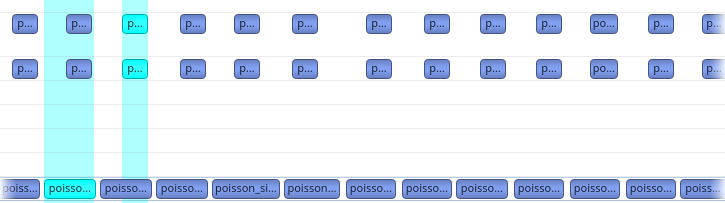
\includegraphics[width=\textwidth]{Ch48Implementation/figures/cudagraphs_before.png}
        \caption{Before CUDA Graphs}
    \end{subfigure}
    \vspace{1cm}
    \begin{subfigure}{\textwidth}
        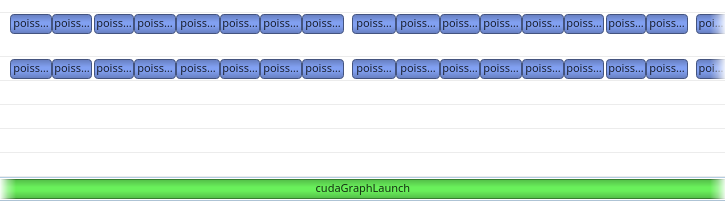
\includegraphics[width=\textwidth]{Ch48Implementation/figures/cudagraphs_after.png}
        \caption{After CUDA Graphs}
    \end{subfigure}
    \caption{Profiler traces of the Poisson kernels before and after CUDA graphs}
    \label{fig:CudaGraphsImpact}
\end{figure}

\begin{figure}
    \centering
    \begin{subfigure}{0.49\linewidth}%
        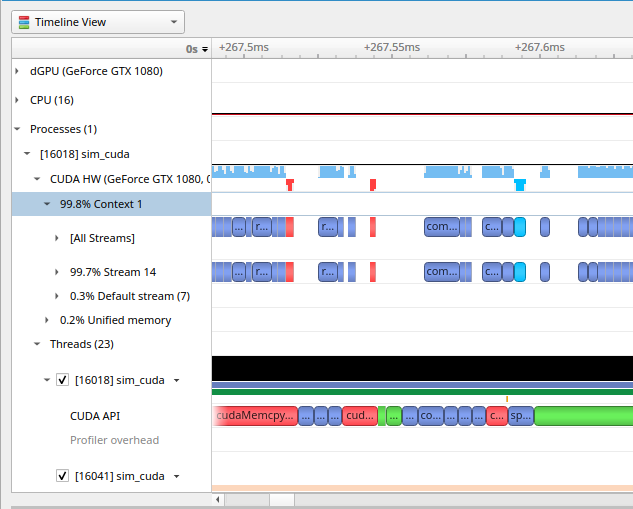
\includegraphics[width=\linewidth]{Ch48Implementation/figures/memcpy_sync.png}%
        \caption{Synchronous Copy}%
    \end{subfigure}%
    \begin{subfigure}{0.49\linewidth}%
        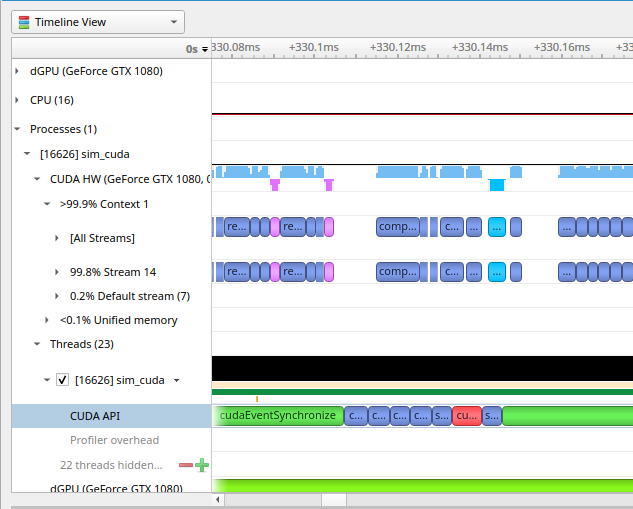
\includegraphics[width=\linewidth]{Ch48Implementation/figures/memcpy_async.png}%
        \caption{Asynchronous Copy}%
    \end{subfigure}
    \caption{Using asynchronous copies for greater efficiency}
    \label{fig:async_copy}
\end{figure}

% Copying the result back to the CPU is done asynchronously, which requires pinned memory to be allocated\todocite{pinned memory}.
% Normal virtual memory can be paged to disk or moved around by the OS, which means there is no reliable location for the GPU to eventually copy data to.
% Pinned memory must be specially allocated, and cannot be moved around, so the asynchronous copy can go ahead as planned.
% If pinned memory were not used the copy to CPU would be synchronous, which would delay the second 

% The profiler showed X when not using pinned memory, as copies to non-pinned CPU memory are synchronous so must wait for the first reduction before enqueueing the second.

% Currently the CUDA program uses the second kernel model, and this is planned to be moved up to the seventh kernel in the future.

% The CUDA program uses the second kernel model. 
% Upgrading to the seventh model was considered, but as the program does not include the residual check, the reductions are infrequent enough (two per tick) that upgrading was not necessary.
% In the future, this may be improved if Poisson residuals were introduced.\todomark{actual future work}
% \todomark{Mention pinned memory here}

\subsection{Usage in Other Layers}
The visualization layer instantiates a \code{VulkanTickedRunner} with \code{CudaBackendV1} to run a visualized simulation.

The command-line layer instantiates a \code{FixedTimeRunner} with any one of the backends to run a headless simulation.

\pagebreak
\section{Visualization Layer}\label{sec:ImplementationViz}
\subsection{Multithreading}
The worker thread is implemented with a \mintinline{cpp}{SystemWorker} class combined with a generic threading system.
% While only one worker thread is ever used in the final program, earlier versions planned to use a few unique workers so a generic system was required.
An \mintinline{cpp}{IWorkerThread} virtual interface is defined and \mintinline{cpp}{IWorkerThread_Impl<Worker>} implements this for a specific \mintinline{cpp}{Worker} class, similar to the Simulation Runners pattern.
% A similar pattern to Simulation Runners is used, where an \mintinline{cpp}{IWorkerThread} virtual interface is defined and a \mintinline{cpp}{IWorkerThread\_Impl<Worker>} class implements this for a specific \mintinline{cpp}{Worker} class.

% The \mintinline{cpp}{IWorkerThread} class works with a \mintinline{cpp}{WorkerThreadController} class.
To kick off the worker thread, a \mintinline{cpp}{WorkerThreadController} writes to a mutex-protected set of input data.
The `work index' of this data is incremented to signal it is new, and a condition variable is signalled to alert the worker thread and begin processing.
Work cannot be enqueued until the thread produces an output, which is sent to the main thread in the same way as before - a mutex is taken to update the output data with the new index, and the condition variable is signalled in case the main thread is waiting for the worker to finish.

\subsection{GPU Work Breakdown}
% \todoref{GPU work breakdown design} showed a coarse breakdown of work between the Viz Compute and Viz Graphics stages, which \cref{fig:VizDataTransform} expands on.
\cref{fig:VizDataTransform} expands on the coarse GPU work breakdown from \cref{sec:Design:Viz:Breakdown}.
Each rectangle represents a piece of memory, and each arrow represents a transformation from input to output via a compute shader, an image layout transfer, or a graphics pipeline.
Most memory is global rather than per-frame, as the system does not run any visualization stages in parallel.
Some per-frame memory is used to allow race-free accesses at record-time.
These buffers allow user interaction, such as moving the particle emitters and setting the quantity ranges, and are highlighted in bold.
% \begin{landscape}
% \thispagestyle{empty}
\pagebreak
\newgeometry{margin=2cm}
\begin{sidewaysfigure}
    \centering
    \makebox[\linewidth][c]{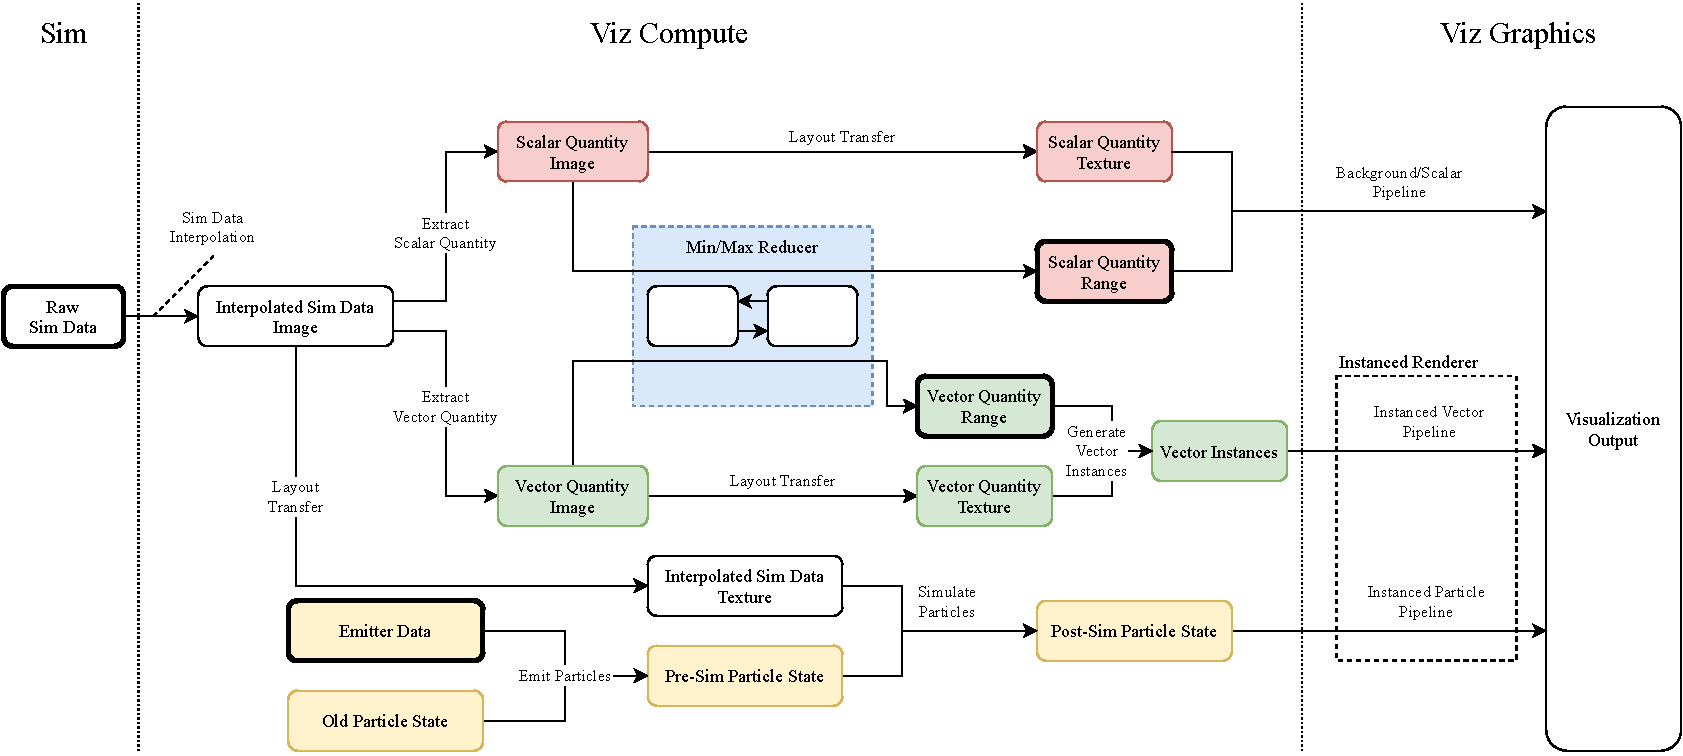
\includegraphics[width=0.9\linewidth]{Ch48Implementation/figures/FinalReport_VizData.pdf}}
    \caption{Data Transformation Diagram showing the data flow for the Visualization}
    \label{fig:VizDataTransform}
\end{sidewaysfigure}
\restoregeometry
\pagebreak
% \end{landscape}

Image layout transfers allow the GPU to optimize access times for an image by changing the format it's stored in.
Images are transferred to the \mintinline{cpp}{ShaderReadOnlyOptimal} layout (listed as `Texture' rather than `Image' in \cref{fig:VizDataTransform}) for efficient sampling at arbitrary points, and kept in the \mintinline{cpp}{General} layout when accessed at 2D data arrays (see \cref{fig:VizImageRead} as a comparison).

Memory barriers (not shown in \cref{fig:VizDataTransform}) are inserted between every compute shader to ensure any required data written from a previous shader is visible to the next shader\cite{TheKhronosGroupVulkanSpec}. % Could also be \cite{MaisterVulkanSyncBlog}
% On top of that, each compute shader requires at least one \emph{memory barrier}, to ensure any data written in previous stages is visible to the next stage.
These memory barriers are quite granular, as shown in \cref{fig:VizMemoryBarrier}.

\begin{figure}
    \centering
     \begin{subfigure}[b]{0.49\textwidth}
         \centering
\begin{glslcode}
uniform readonly image2D resultImage;
 // = (u, v, p, isfluid);

// Specify the exact pixel location
ivec2 pxIdx = ivec2(200, 450);
vec4 data = imageLoad(simDataImage, pxIdx);
\end{glslcode}
\caption{Directly}
        %  \label{fig:vizimageLoad}
     \end{subfigure}
     \hfill
     \begin{subfigure}[b]{0.49\textwidth}
         \centering
\begin{glslcode}
uniform sampler2D simDataSampler;
 // = (u, v, p, isfluid);
 
// 50% across, 20% up the image
vec2 sampleAt = (0.5, 0.2);
vec2 velocity = texture(simDataSampler, sampleAt).xy;
\end{glslcode}
\caption{With a Sampler}
        %  \label{fig:vizimagesample}
     \end{subfigure}
  \caption{Reading from an image directly vs. using a sampler.}
    \label{fig:VizImageRead}
\end{figure}
\begin{figure}
    \centering
    \begin{cppcode}
// Make ShaderWrites from the ComputeShader stage available + visible to 
//      IndirectCommandReads in the DrawIndirect stage
fullMemoryBarrier(computeCmdBuffer,
    vk::PipelineStageFlagBits::eComputeShader, vk::PipelineStageFlagBits::eDrawIndirect,
    vk::AccessFlagBits::eShaderWrite, vk::AccessFlagBits::eIndirectCommandRead);
// Make TransferWrites from the Transfer stage available + visible to the
//      ShaderReads in the ComputeShader phase.
fullMemoryBarrier(computeCmdBuffer,
    vk::PipelineStageFlagBits::eTransfer, vk::PipelineStageFlagBits::eComputeShader,
    vk::AccessFlagBits::eTransferWrite, vk::AccessFlagBits::eShaderRead);
    \end{cppcode}
    \caption{Example showing the granularity of Memory Barriers.}
    \label{fig:VizMemoryBarrier}
\end{figure}

\pagebreak
\begin{figure}[t]
    \centering
    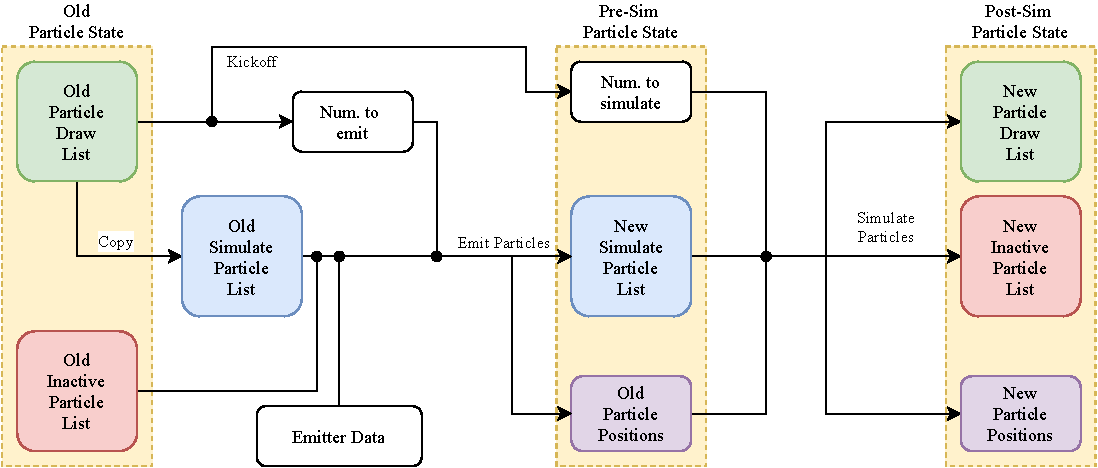
\includegraphics[width=\linewidth]{Ch48Implementation/figures/FinalReport_VizData_Particles.pdf}
    \caption{Breakdown of particle-related GPU work}
    \label{fig:VizDataParticles}
\end{figure}
The particle system implentation in \cref{fig:VizDataTransform} is a simplified view for compactness, \cref{fig:VizDataParticles} shows a full breakdown of this subsystem.
This maintains three growable/shrinkable lists, plus a buffer containing particle positions.
\begin{enumerate}
    \item The Draw list, a list of particle indices to draw on screen
    \item The Inactive list, a list of inactive particle indices
    \item The Simulate list, a list of particle indices which take part in Simulation.
\end{enumerate}
The previous Draw list is the authority on which pariticles currently exist, and is used for the Kickoff shader to determine how many particles will be emitted/simulated\footnote{This isn't known at record time, because the last frame may still be simulating the particles}.
It is also copied into the Simulate particle list, which is grown by the Emit Particles shader.
The particles are then moved by the Simulate Particles shader as shown in \cref{sec:Research:Viz:Particles}.
These particles are added to the inactive list if out-of-bounds, and the new Draw list otherwise.
% adding particles to the inactive list if they move out of the simulation bounds, and moving all other particles to the new Draw list.

\subsection{Safe CPU/GPU Communication}\label{sec:Impl:Viz:CPUGPUSafety}
Unlike CUDA, the Vulkan API does not provide any means of type-safety when communicating between the CPU and GPU.
If the GPU expects data in a specific structure, it is the API user's job to create data that fits this structure.
A naive solution might be to keep a C++ structure definition and a GLSL structure definition, and assume that one matches the other.
This is error prone as the structures are not automatically kept in sync - if one changes, the other will not, and communication will break down.
This project's approach is to create a GLSL file defining all interoperable structures (\texttt{structures.glsl}), and then include it into a C++ header with some extra code to define GLSL types correctly.
Both sides will now use the same structure definitions, which are all defined in exactly one place.
All GLSL code uses the \texttt{std430} memory layout rules, which closely matches the C++ memory layout, so the structures can be passed directly from the CPU to the GPU safely.

\subsection{Usage in Other Layers}
The \mintinline{cpp}{VulkanSimApp} class is instantiated by the command-line layer to run the visualization.

\pagebreak
\section{Command-Line Layer}
The command-line layer is implemented with a set of subapps, each implemented by a separate virtual class satisfying an interface \code{ISubApp}.
Virtual inheritance was chosen here because it is convenient and not in a performance-critical area.
Each ISubApp instance is used to create a CLI11 subcommand with some input arguments, then CLI11 parses the command-line arguments and runs a callback on the selected subapp.
These subapps then invoke other layers of the system to complete their execution.
% !TEX root =  ../FinalReport.tex

\chapter{Project Management}
\label{sec:ProjectManagement}

To ensure a smooth development process, all research and implementation was planned ahead of time.
This chapter details these plans including a complete schedule, the development methodology used, the tools used, and the potential risks and associated contingencies.

\section{Software Development Methodology}
Plan-driven solutions depend on a rigid specification being completed before development\cite{modules:CS261}, which did not fit with the more abstract goals of the visualization portion.
Additionally, some of the main advantages of plan-driven approaches only apply when introducing new team members and handling large teams.
Neither scenario applies here, as only one person is undertaking active development.
For these reasons, an Agile approach was taken with a development cycle completing every two weeks.
The goals for each development cycle were documented using Trello.

It was planned that the supervisor would be contacted every week with the current status of the project and the progress made in the current cycle.
These contacts would either take place over e-mail if there were no pressing questions to ask, and otherwise take place on Microsoft Teams.
Unfortunately, this did not happen for the first few weeks, as other work was vying for attention and preventing project work from taking place.
This was resolved in Week 5, and from then on there was frequent email correspondence.

\section{Project Timeline}
The project was split into multiple tasks to schedule it effectively.
These tasks are scheduled on both a Gantt Chart in \cref{fig:project schedule gantt}, and as a table in \cref{tab:project schedule table}.
The timeline has been well followed, and this schedule has been left unchanged over the course of the project. 

No programming was scheduled over the Christmas break to allow time to be spent on other assignments.
%time on the other courseworks the researcher will have due.
The development of the visualization was scheduled concurrently with optimizing the simulation, in case some strides in visualization required extra optimizations to run in real-time.
While not strictly required, some optimizations were developed in this time to push performance further.
% This was not strictly the case, but some optimizations were developed in this time period to push performance further.
A Code Freeze was set for Week 22, to focus the researcher entirely on the presentation.
%where development is then completely focused on the presentation.

\begin{figure}[ht]
    \centering
    % \begin{tikzpicture}
    % \node[inner sep=0pt] (gantt) at (0,0)
    % {\includegraphics[width=1.0\linewidth]{Presentation/presentation_gantt.pdf}};
    % \draw[line width=0.5mm] (5.4, -1.25) -- ++(0, 3) node[anchor=north east,align=right,fill=white] {Code Freeze};
    % \node[text width=1.2cm,minimum height=2.35cm,fill opacity=0.5, fill=gray, font=\small,align=center, text opacity=1] at (-0.1,-0.02) {Christmas break and other work};
    % \end{tikzpicture}
    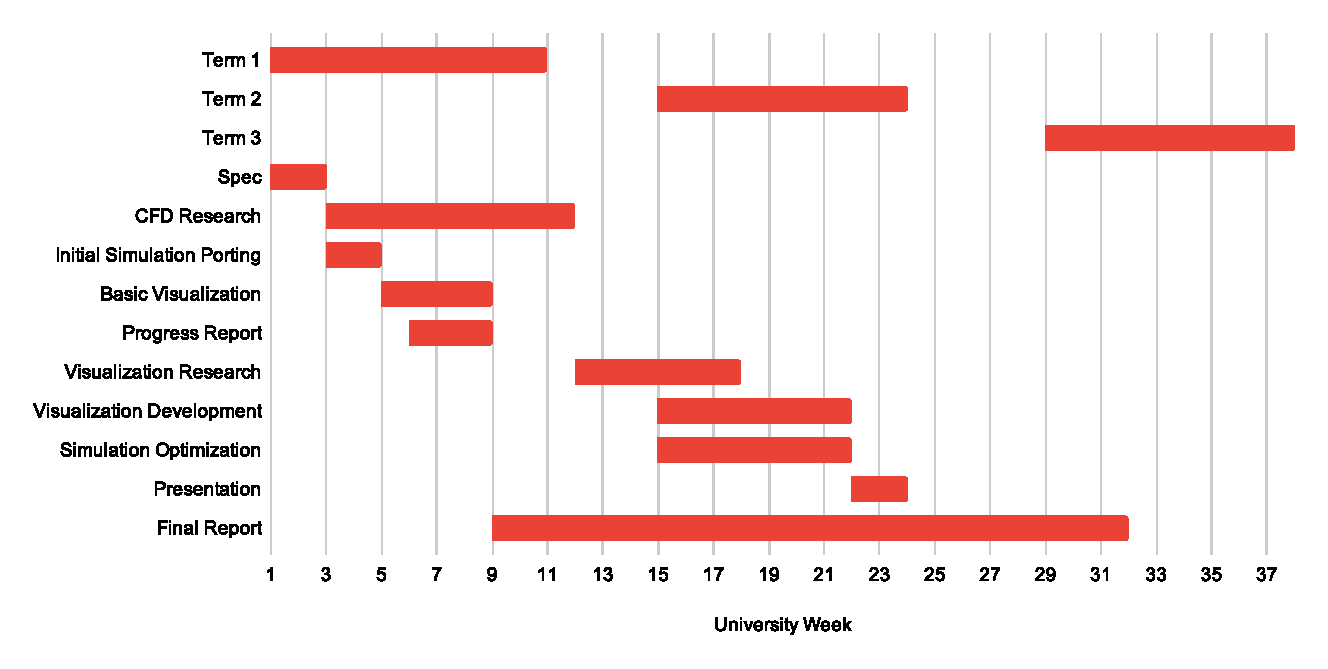
\includegraphics[width=\linewidth, trim={0 0 0 2.7cm},clip]{Ch50ProjectManagement/cs311_gantt_chart.svg.pdf}
    \caption{Project Schedule as a Gantt Chart}
    \label{fig:project schedule gantt}
\end{figure}

\begin{table}[ht]
    \centering
    \begin{tabular}{l|c|c}
    \textbf{Task} & \textbf{Start Week} & \textbf{End Week} \\
    \hline
    Spec & 1 & 3 \\
    CFD Research & 3 & 12 \\
    Initial Simulation Porting & 3 & 5 \\
    Basic Visualization & 5 & 9 \\
    Progress Report & 6 & 9 \\
    Visualization Research & 12 & 18 \\
    Visualization Development & 15 & 22 \\
    Simulation Optimization & 15 & 22 \\
    Presentation & 22 & 24 \\
    Final Report & 9 & 32 \\
    \end{tabular}
    \caption{Project Schedule Tasks}
    \label{tab:project schedule table}
\end{table}

\section{Tools}
\label{sec:ProjManagementTools}
\shell{gcc 8} was used to compile the program.
This version had stable support for the C++14 and C++17 standards, allowing modern techniques to be used in the program.
CMake was used to handle building the program source files.
Versions 3.8 and up support CUDA as a first-class language, which simplified the compilation process.
% The CLion IDE is used on the researcher's personal machine, as the researcher is familiar with the other IDEs in this family.
% If DCS machines are used, GNU Emacs will be used to edit files instead.

Git was used for source control, synchronized to a private GitHub repository to avoid data loss.
The researcher used the CLion IDE to develop the program, which simplified building the program and interacting with source control.

\LaTeX{} was used to create the various reports and non-program deliverables required by the project, which were hosted on Overleaf so they could be compiled on Windows and Linux without installing a \LaTeX{} environment.

%Trello
Trello was used to track bugs and upcoming features in each development cycle.
Google Drive was used to host other documents, e.g. scanned notes, that were created during development.

\section{Risk Management}
% As the project continues, there are risks that may impede progress and even prevent the project from succeeding.
When progressing through the project, there were risks that could impede progress and even prevent the project from succeeding.
Being aware of these risks allowed them to be predicted ahead of time, avoided, or in the worst case mitigated once they arrived.
Risk can be calculated with the following equation, where Severity and Likelihood are graded between 1 and 5.
\begin{equation*}
    Risk = Severity * Likelihood
\end{equation*}

Of these risks, Illness and Other Pressures were encountered during development.
Both were mitigated quickly and did not cause a large delay.
% Some of these risks were encountered, including a new risk (Other Pressures) which was not accounted for in the Specification.
% Thankfully this risk did not cause a large delay.

\subsection{Misscheduling}
It may have been possible that the features outlined in \cref{sec:Requirements} were too great to be implemented in the allotted time.
In that case, the quality of work could have to be reduced to meet deadlines, or the schedule would need to be changed.
This is especially relevant to the Visualization portion of the project, which was not fully planned until the research was completed.

\textbf{Risk} = 2 * 2 = 4

\textbf{Avoidance:}

\hspace{20pt}Previous projects were used as a reference to predict how long implementing features will take, and inform the schedule.
As new Visualization features were discussed, the impact on scheduling they each have were considered.

\textbf{Contingency:}

\hspace{20pt}The scope of the project could have been reduced to allow the report to be completed in time.
A ``code freeze'' was implemented close to the presentation deadline to ensure enough time is spent polishing the presentation and report.

\subsection{Other Pressures}
While the project schedule may have been well estimated based on the work required for the project, the amount of work required for other modules was larger than expected.
This manifested in Term 1, where the researcher took more modules than usual. 
Additionally, the removal of in-person lectures due to COVID-19 led to a lack of overall structure, which made organizing the other work more difficult.
This did not impact the schedule.

\textbf{Risk} = 2 * 1 = 2

\textbf{Avoidance:}

% A more balanced set of modules between Term 1 and Term 2 could have helped resolve this, however on the other side of the coin the researcher had fewer modules in Term 2.
% Balancing modules between Term 1 and Term 2 could have resolved this, but as Term 2 had fewer mo
% Next term the researcher will try to maintain a schedule for working on other module content, which should make up for a lack of in-person lectures.
\hspace{20pt}This could have been avoided by better balancing the modules between Term 1 and Term 2, but on the flip-side having fewer modules in Term 2 allowed for more project work to be completed.

\textbf{Contingency:}

\hspace{20pt}As before, the scope of the project could have been reduced to allow the report to be completed in time.
If module work took more time than expected by week 20, the code freeze could have been pulled forwards to week 20 or 21 to spend more time on the presentation.


\subsection{Loss of Hardware Access}
As noted in \cref{sec:Requirements_HardwareSoftware}, a GPU is required for the project to be tested and developed.
The main development environment was the researcher's personal computer, which has a suitable GPU.
However, if this computer were to break down or be stolen, there was no readily available alternate environment.
Under normal circumstances, the Department of Computer Science labs would be used instead, as they also have suitable GPUs, but the virus situation prevented this.

\textbf{Risk} = 5 * 1 = 5

\textbf{Avoidance:}

\hspace{20pt}Not possible.

\textbf{Contingency:}

\hspace{20pt}Student insurance could have been used to purchase a new GPU/computer if it is stolen.
Failing this, the DCS clusters could be used, but these would likely have high contention from other students who need to use GPUs remotely.

\subsection{Illness}
It is always prudent to consider the possibility that the stakeholders may fall ill and be unable to work on the project for some time.
This was exacerbated by the situation with COVID-19, making potential illnesses more dangerous than usual.

This risk manifested during Week 7 and delayed work on the project by three days.
However the bulk of the current work had been completed by that point, so this module was not affected.%other modules were affected.

\textbf{Risk} = 4 * 2 = 8

\textbf{Avoidance:}

\hspace{20pt}Not possible.

\textbf{Contingency:}

\hspace{20pt}The schedule would need to be changed to account for the lack of time spent working.
Some requirements could be reduced or removed entirely.


\chapter{Testing \& Success Measurement}\label{sec:Testing}
In order to measure the degree of success a project achieves, testing must be performed to verify the behaviour of the program is correct.
This covers testing the functionality of individual units of the program (unit testing), testing how those units interact with each other (integration testing), and validating the behaviour of the overall system against the functional and non-functional requirements\todocite{https://reqtest.com/testing-blog/different-levels-of-testing/}.
This section also defines the means of Success Measurement for some non-functional requirements, which are then measured and evaluated in subsequent sections.% The codebase does not lend itself well to automatic testing, as most components have behaviour that's too difficult to automatically verify (such as automatic memory management, or the entire visualization).
% \todomark{More on explanation of Testing chapter}

\section{Unit Tests}
The first layer of testing splits the program into `units', that are independent of each other, which are individually tested before combining them with other units in the system.
In some systems it is practical to automate these tests, but this was not pursued for this system as the behaviour is generally too complex to be automatically verified.

Helpfully the program is already split into subcommands at the command-line level (\cref{sec:DesignSubcommands}), which can all be tested individually.
% The \texttt{compare}, \texttt{renderppm}, and \texttt{fixedtime} subcommands can each be tested completely independently of other.
Because the file format is the same as the original coursework, the original input file can be used to test comparisons (\texttt{compare}), simple visualization (\texttt{renderppm}), and both simulations (\texttt{fixedtime} and \texttt{run}).
These commands all have equivalents in the original coursework, which provides a basis for validating correctness.
The \texttt{makeinput} subcommand, which creates a new input file based on an image, can be tested by passing the resulting input file to other known-functional subcommands and checking their behaviour.
This provides a coarse view of system functionality, but a finer level of detail can be obtained by testing individual code components.

Unit-testing this particular codebase is difficult because many components are dependent on other components - for example, the visualization components use data gathered from the simulation output, which is impractical to extract for the sake of testing individual components.
It is easier to just test the complete visualized simulation while assuming the simulation itself is correct.
In other cases, unit behaviour may be impractical to directly model or verify: the automated resource management classes are difficult to test individually as the creation/destruction of the resources they manage cannot be directly checked.
However there are some areas where the codebase can be effectively unitized, the most prominent of which is the simulation itself.

The simulation is split into stages, which are effectively independent code units.
Each unit depends on the output of the previous unit, so they cannot be tested independently, but if the rest of the simulation units are known to be correct then an individual unit can be tested.
This technique was used during development to ensure the CUDA simulation was consistent with the CPU version.

Overall, while unit tests are not always suitable for elements of the codebase, they are helpful at a coarse level.
The final set of unit tests are shown in \cref{tab:unittests}.

\section{Integration Testing}
Once the program units have been individually tested, Integration Testing tests if the units can interface with each other correctly.
Again the subcommands are treated as units, and testing is performed by passing an output from one subcommand as the input to another.
In this program only the \texttt{makeinput} and \texttt{fixedtime} subcommands produce output, so their output is exhaustively tested against the other commands.
At the codebase level some previous unit tests can be counted as integration tests:
the headless simulation functions as an integration test for the Memory and Simulation layers, and the visualized simulation tests the integration between the Simulation and Visualization layers.

The C++ type system ensures that low-level connections between CPU code use the correct types, making integration testing at this level redundant.
Moving data between the CPU and GPU is more complicated, but the elements put in place in (\cref{sec:Impl:Viz:CPUGPUSafety}) and the Vulkan validation layers (\cref{sec:Impl:CodeSafety}) ensure that any integration errors are caught when simply running the program in Debug mode.

The Integration tests are shown in \cref{tab:integration_tests}.



\section{System Testing}
This final layer of testing determines if the program upholds the functional and non-functional requirements set out in \cref{sec:Requirements}.
Some functional requirements such as \cref{req:VizPauseResume} require in-depth checks of the visualization not suitable for other layers, so are tested here.
The System Tests specified in \cref{tab:sys_tests_func} cover all such tests, and combined with the previous layers of tests prove that the system meets the functional requirements.

Many non-functional requirements can be tested directly: \cref{reqN:Resources} is tested with external programs \texttt{valgrind} and \texttt{cuda-memcheck}, \cref{reqN:Documented,reqN:UsageGuide} are tested by simply inspecting the program and source files, \cref{reqN:DCSCompile} is tested by attempting to compile + run the program on DCS systems.
A few require a large amount of data collection, or at least careful attention to detail.
% The others need special care and extra specification to measure qualitatively.
% The nonfunctional tests (\todoref{system tests nonfunctional}) handle the non-functional requirements.
% Some of these tests are more complex and require more data to evaluate them.
These tests are specified in \cref{tab:sys_tests_nonfunc}.
All gathered data is specified in the next subsection, and then the results are shown in \cref{sec:Results}.

% \newcommand{\testsuccess}{\symbol{"2B45}}
% \newcommand{\testfail}{\symbol{"2718}}

\newcommand{\testsuccess}{\cmark{}}
\newcommand{\testfail}{\xmark{}}

% \pagebreak
% \newgeometry{margin=2cm}
% \begin{sidewaysfigure}
%     \centering
%     \makebox[\linewidth][c]{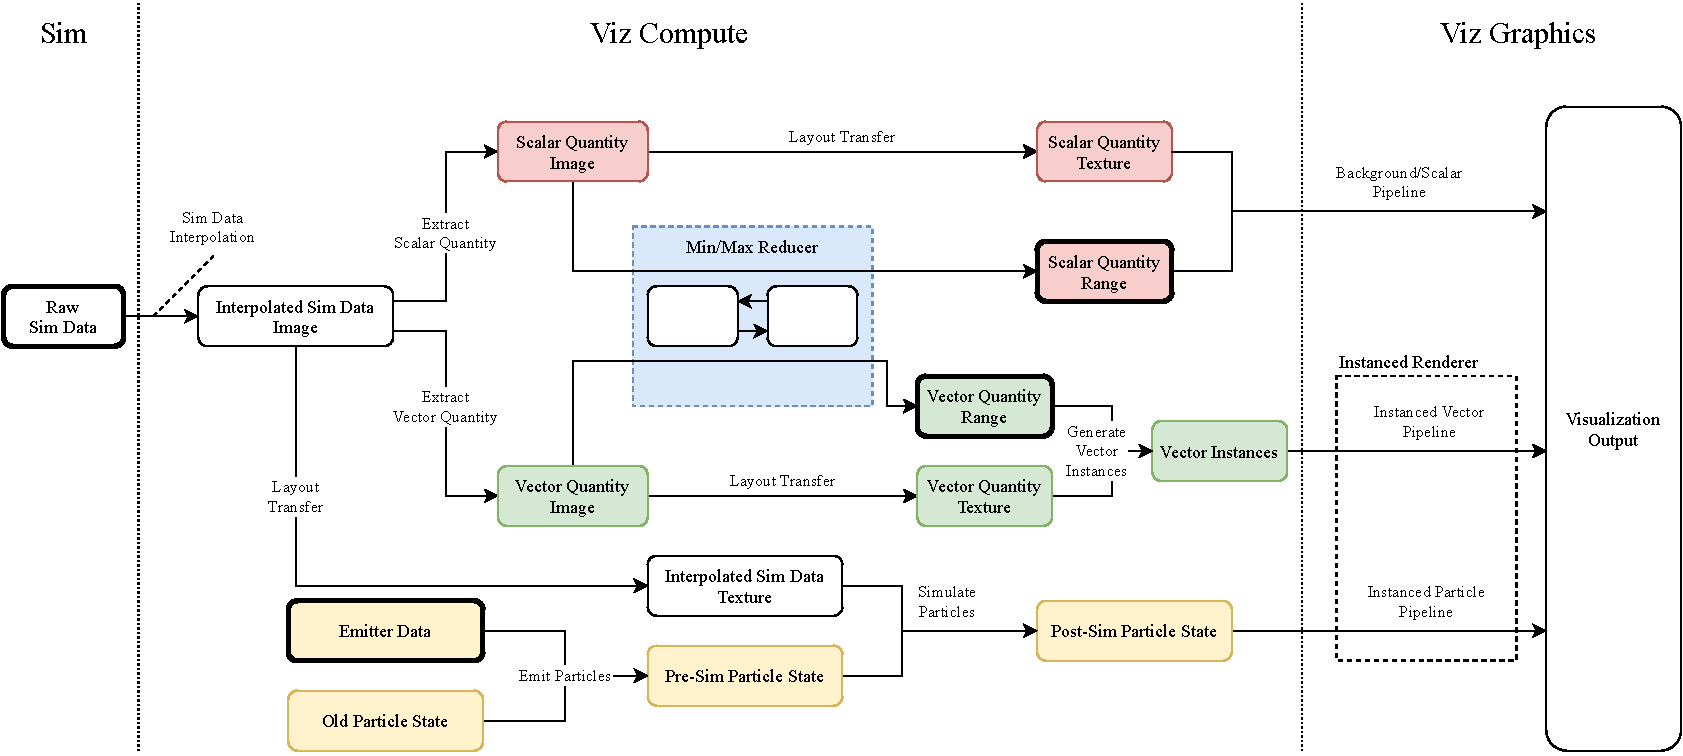
\includegraphics[width=\linewidth]{Ch48Implementation/figures/FinalReport_VizData.pdf}}
%     \caption{Data Transformation Diagram showing the data flow for the Visualization}
%     \label{fig:VizDataTransform}
% \end{sidewaysfigure}
% \restoregeometry
% \pagebreak

\begin{sidewaystable}
    \centering
    \begin{tabular}{ll|c|c|c}
        ID & Description & Expected & Output & Result \\
        \hline
        \newtest{}\label{test:unit:compare:identical} & \shell{compare}: identical states & No difference & No difference & \testsuccess{} \\
        \newtest{}\label{test:unit:compare:different} & \shell{compare}: Original input to original target output & Some difference & Some difference & \testsuccess{} \\
        \newtest{}\label{test:unit:renderppm} & \shell{renderppm}: render state vorticity & Equal to original program & Equal to original program & \testsuccess{} \\
        \newtest{}\label{test:unit:makeinput} & \shell{makeinput}: generate an input file from a PNG & Valid simulation state & Valid simulation state & \testsuccess{} \\
        \newtest{}\label{test:unit:fixedtime} & \shell{fixedtime}: simulate from an input state for 25 seconds. & Valid simulation state & Valid simulation state & \testsuccess{} \\
        \newtest{}\label{test:unit:run} & \shell{run}: visualize a simulation from an input state for 25 seconds. & Valid simulation state & Valid simulation state & \testsuccess{} \\
    \end{tabular}
    \caption{Unit Tests}
    \label{tab:unittests}
\end{sidewaystable}


\newcommand{\integtest}[2]{\shell{#1} & $\xrightarrow{}$ & \shell{#2}}
\newcommand{\successoutput}[1]{#1 & As expected & \testsuccess{}}

\begin{sidewaystable}
    \centering
    \begin{tabular}{lccl|p{0.4\linewidth}|m{0.2\linewidth}|c}
        ID & \multicolumn{3}{l}{Integrated Modules} & Expected & Output & Result \\
        \hline
        \newtest{}\label{test:intg:input:render} & \integtest{makeinput}{renderppm} & \successoutput{Valid render image with the same obstacle squares as the initial image.} \\
        \newtest{}\label{test:intg:input:cmp} & \integtest{makeinput}{compare} & \shell{compare} runs successfully & \shell{compare} ran successfully & \testsuccess{} \\
        \newtest{}\label{test:intg:input:sim} & \integtest{makeinput}{fixedtime} & \successoutput{Valid simulation output with the same obstacle squares as the initial image.} \\
        \newtest{}\label{test:intg:input:viz} & \integtest{makeinput}{run} & \successoutput{Visualization of a simulation with the same obstacle squares as the initial image.} \\
        \hline
        \newtest{}\label{test:intg:sim:render} & \integtest{fixedtime}{renderppm} & \successoutput{Valid render image with the same obstacle squares as the initial state.} \\
        \newtest{}\label{test:intg:sim:cmp} & \integtest{fixedtime}{compare} & \shell{compare} runs successfully & \shell{compare} ran successfully & \testsuccess{} \\
        \newtest{}\label{test:intg:sim:sim} & \integtest{fixedtime}{fixedtime} & \successoutput{Valid simulation output with the same obstacle squares as the initial state.} \\
        \newtest{}\label{test:intg:sim:viz} & \integtest{fixedtime}{run} & \successoutput{Visualization of a simulation with the same obstacle squares as the initial state.} \\
    \end{tabular}
    \caption{Integration Tests}
    \label{tab:integration_tests}
\end{sidewaystable}

\begin{sidewaystable}
    \centering
    \begin{tabular}{ll|p{0.35\linewidth}|m{0.2\linewidth}|c}
        ID & Description & Expected & Output & Result \\
        \hline
        \newtest{}\label{test:sys:sim:gpu} & \texttt{fixedtime}: GPU Simulation & \successoutput{Simulation backend can be set to CUDA} \\
        \newtest{}\label{test:sys:run:gpu} & \texttt{run}: GPU Simulation & \successoutput{Simulation backend can be set to CUDA} \\%Can visualize a simulation running on the GPU
        \hline
        \newtest{}\label{test:sys:run:pause} & \texttt{run}: Test pausing/resuming the simulation & \successoutput{Simulation can pause/resume while the visualization is running} \\
        \newtest{}\label{test:sys:run:save} & \texttt{run}: Test saving the simulation state & Simulation state can be saved while visualizing & Couldn't save state while running & \testfail{} \\
        \newtest{}\label{test:sys:run:manip} & \texttt{run}: Test moving the particle emitters & \successoutput{Particle emitters can be moved while the simulation is running} \\
        \newtest{}\label{test:sys:run:lockedFPS} & \texttt{run}: Can run with a fixed framerate & Framerate can be fixed at some value & Framerate was fixed at 120FPS and did not change & \testsuccess{} \\
        \newtest{}\label{test:sys:run:flatoutFPS} & \texttt{run}: Can run with an unlocked framerate & Framerate can be unlocked & Framerate was not locked and varied between 750-800FPS & \testsuccess{} \\
        \newtest{}\label{test:sys:run:layerPerms} & \texttt{run}: All Viz layers work as expected. & \successoutput{All layer combinations can be used, all layers function as described in \cref{sec:Requirements}.} \\
        \newtest{}\label{test:sys:run:autorange} & \texttt{run}: Test auto-range functionality & \successoutput{Auto-ranged Scalar and Vector quantities display all values in the sim boundary.} \\
        \newtest{}\label{test:sys:run:colors} & \texttt{run}: Test changing colors & \successoutput{All colors used in the simulation should be modifiable} \\
        \newtest{}\label{test:sys:run:validation} & \texttt{run}: Check Vulkan validation & \successoutput{No Vulkan validation errors in Debug mode} \\
    \end{tabular}
    \caption{System Tests (Functional)}
    \label{tab:sys_tests_func}
\end{sidewaystable}

\begin{sidewaystable}
    \centering
    \begin{tabular}{lp{0.2\linewidth}|p{0.4\linewidth}|m{0.2\linewidth}|c}
        ID & Description & Expected & Output & Result \\
        \hline
        \newtest{}\label{test:sys:sim:large} & \texttt{run}: Large Simulation & \successoutput{Simulation can run on a 4096x4096 input.} \\
        \newtest{}\label{test:sys:sim:valgrind} & \texttt{run}: No CPU memory leaks & Visualization run under \texttt{valgrind} should have no program-controlled memory leaks. & See \cref{sec:Results:Sim:Mem,sec:Results:Viz:Memory} & \testsuccess{} \\
        \newtest{}\label{test:sys:sim:cudamemcheck} & \texttt{run}: No CUDA memory leaks & Simulation run under \texttt{cuda-memcheck} should have no program-controlled memory leaks. & See \cref{sec:Results:Sim:Mem,sec:Results:Viz:Memory} & \testsuccess{} \\
        \newtest{}\label{test:sys:run:pipeline} & \texttt{run}: High GPU Utilization & Nsight Systems profiler output should show maximum achievable GPU utilization\footnote{100\% may not be possible due to other programs using the GPU} & See \cref{sec:Results:Sim:Efficiency,sec:Results:Viz:Efficiency} & \testsuccess{} \\
        
        
        \newtest{}\label{test:sys:sim:speed} & \texttt{fixedtime}: Simulation is faster than original simulation & CUDA simulation should run 2x faster than the original simulation on the original input. &See \cref{sec:Results:Sim:Speed} & \testsuccess{} \\
        \newtest{}\label{test:sys:sim:accuracy} & \texttt{fixedtime}: Simulation produces similar results to original simulation &
        CUDA simulation solver residual should be within 5\% of adapted CPU backend.
        & See \cref{sec:Results:Sim:Accuracy} & \testsuccess{} \\
        % CUDA simulation output should be within $10^-10$ of the adapted CPU backend output. & See \cref{sec:Results:Sim:Accuracy} & \testfail{} \\

        \newtest{}\label{test:sys:run:highFPS} & \texttt{run}: Can run at high framerate & Visualization can run at >30FPS in some case & Simulating the original input at N=100 runs at \~800FPS. & \testsuccess{} \\
        \newtest{}\label{test:sys:run:vizSpeed} & \texttt{run}: Visualization features are faster than simulation & See \cref{sec:Testing:SuccessMeasurement} & See \cref{sec:Results:Viz:Speed} & \testsuccess{} \\
        \newtest{}\label{test:sys:run:dcsComp} & Try to compile on DCS systems & Should be able to compile and run the simulation on elements of the DCS system. & Successfully compiled non-CUDA sim on DCS. & \testsuccess{} \\
    \end{tabular}
    \caption{System Tests (Non-Functional)}
    \label{tab:sys_tests_nonfunc}
\end{sidewaystable}


\subsection{Success Measurement}\label{sec:Testing:SuccessMeasurement}
\cref{test:sys:sim:valgrind,test:sys:sim:cudamemcheck} test the memory usage of the system.
The most important kind of error they can detect are memory leaks, where memory is allocated without being released, leading to the program taking up memory it does not need anymore.
While it is important to avoid memory leaks in all cases the most important variation is continuous memory leaks, where memory is continuously leaked over and over, or large leaks of sizes larger than 100MB.
Single small leaks are less concerning, as they should not impact the rest of the system greatly.
The programs used to find these leaks may themselves be bad at recognizing allocation/freeing\cite{ValgrindProblemsBlog}, and lead to false-positives.
Care must be taken when evaluating their results.
\cref{test:sys:sim:speed,test:sys:sim:accuracy} evaluate the speed and accuracy of the CUDA-based simulation backend vs. the adapted CPU backend.
The accuracy is measured by comparing the output of equivalent simulations on the original CS257 input state.
Other states were tested, but any newly generated states with obstacles proved to be unstable and produce Not-a-Number outputs on both backends.
The simulation speed is tested on the original CS257 input state, then behaviour at scale is tested on custom generated states with no obstacles.
Obstacle configuration does not affect time-per-tick, so time-per-tick will be a representative value and equal for any state of the same size.
This would not be suitable for accuracy tests, as having no obstacles greatly reduces the complexity and would likely produce disproportionately high accuracy values.

As there is no visual component to the simulation tests, the program is run from a terminal without running the X windowing system.
Combined these tests should give a complete picture of how the CUDA simulation's speed and accuracy will scale, and be enough to evaluate the requirements in context.

% To account for all possible factors, results were gathered for many permutations of variables. \todomark{(shown in variable table?)}
% Two input files are used: the original ACA input file (660x120), and a custom 1024x512 image representing \SI{128}{\metre}x\SI{64}{\metre}s of physical space (see \todoref{figure of circles}).
% Larger images are less likely to fit in cache, so accentuate the impact of memory usage on the algorithm.
% Four different simulation configurations are used, which only differ in Poisson iteration count: 100 (matching the original), 200, 300, and 1000.
% Higher iteration counts ensure the Poisson stage dominates the time taken.
% Each permutation is then run for simulations of 10, 25, and 50 seconds to determine the impact of longer simulations on accuracy.
% To measure the time taken for each test five measurements are taken, the fastest and slowest times are removed, and the three remaining results are then averaged.
% The similarity between tests on different backends is measured using the \texttt{compare} tool, and the Poisson residual for each output is found with a small utility that computes the Poisson RHS (see \cref{sec:Research:SimulationTick}) then immediately determines the residual using the CPU backend.


\cref{test:sys:run:vizSpeed} evaluates the speed of individual visualization features vs. the simulation.
As the time taken to run a simulation tick can be variable based on the input, these visualization speeds are compared to the time allotted to the target 60FPS, i.e. \SI{16.6}{\milli\second}.
These visualization times are measured using the frame-time counter in the GUI (\todoref{example of GUI?}), which measures the average time taken to present the last 32 frames.
First, the time taken to render a frame with no visualization features is taken.
Each feature is then individually enabled, brought to the worst-case scenario (using auto-range where applicable, and rendering the maximum amount of instances where applicable), then the average frame-time is taken.
To ensure the results are not affected by external sources, the program is run in unlocked framerate mode with no other programs running on the system.
This is also the case for the GPU utilization test (\cref{test:sys:run:pipeline}).

These results are shown in \cref{sec:Results}, and then evaluated along with the rest of the test outcomes in \cref{sec:Evaluation}.
% !TEX root =  ../FinalReport.tex

\chapter{Conclusion}
\label{sec:Conclusion} 
% Why was this project worth doing? 

% What’s the contribution of your project? 

% What is its “technical strength”? 

% (Why was this a challenging project suitable to your degree?) Why should your project be considered a success? 


This project aimed to create a GPU fluid simulation and real-time in-situ visualization program, which required substantial research on fluid simulations, optimizing large parallel computation on GPUs, and various visualization methods.
% Implementing the program required knowledge of C++, Vulkan, and CUDA; an in-depth understanding of the complex underlying details of each, including their handling of memory; and an effective high-level design.
The implementation required knowledge of C++, Vulkan, and CUDA; an in-depth understanding of the complex underlying details of each, including their handling of memory; and an effective high-level design.
%that separated the code into manageable layers.
On top of this, the project was well scheduled, allowing all core features to be implemented while allowing enough time for the associated reports and presentation to be developed.
Rigorous testing was undertaken to ensure the program met the requirements, and the program passed with flying colours.
The behaviour of the simulation at scale was measured, producing interesting findings and paving the way for future work in the area.
Overall, the project has been a success.

\section{Summary}
% Novelty of in-situ realtime visualization
% The full in-situ visualization is a very large program, using over 8.5 thousand lines of custom code (excluding external libraries, comments, whitespace), which is impressive in its own right.
The full in-situ visualization is a very large program, with over 8.5 thousand lines of custom code, which is impressive in its own right.
It also brings novelty as an accurate simulation/visualization that runs in real-time, rather than rendering a visualization to disk for later viewing or rendering a static simulation state.
% By using approaches from the games industry for efficient visualization, the visualization 
It uses the high-performance Vulkan rendering API, which other toolkits have been slow to adopt\footnote{VTK has a Vulkan branch at \url{https://gitlab.kitware.com/ken-martin/vtk/-/tree/vulkan/Rendering/Vulkan}, which hasn't been updated since August 2020.}.
Along with the up-and-coming Datoviz library\cite{Datoviz}, it is a step forwards to bring Vulkan-level performance to the wider visualization community.

Porting the simulation to CUDA is not a new work, but it was still a significant undertaking for the researcher and required extra thought to adapt to a tightly-coupled visualization.
Gathering results at different scales demonstrated the upper limit of GPU throughput, and empirically showed the importance of cache-friendliness in GPU algorithms.
It is certainly a good starting point for future work in this space.

\section{Reflection}
% A large contribution to the project's success were the development practices used.
Completing the project successfully relied on using good development practices.
During Term 2 extensive notes were taken while solving bugs and designing the rest of the program, ensuring all notable choices could be documented in this report and the presentation.
Using Git branches to develop multiple features separately prevented confusion when working with the code, and maintaining a `master' branch ensured that an up-to-date bug-free version of the program was always available.
This project also tied in the researcher's prior knowledge from other areas, such as memory models, caches, and functional programming.
% The primary focus of the project was the GPU, but knowledge from other areas was also helpful %when applicable knowledge from other areas 
% This project took advantage of the researcher's prior GPU knowledge, but also utilized many of the researcher's other skills, such as working with memory models, caches, and functional programming.

While the project as a whole was successful, some small elements could have been better executed.
Third-party libraries were used in places, most notably for the GUI, but were not used in the low-level memory management or other Vulkan code.
For Vulkan specifically, using the Vulkan Memory Allocator library\cite{GPUOpenVMA} would have allowed for easier memory allocation.
Other Vulkan wrappers and tools, such as the codebase developed by Sascha Willems for their Vulkan samples\cite{SaschaWillemsVulkan}, may have made certain actions less cumbersome.

A common pattern encountered when implementing new code was to design for a larger system than necessary.
For example, when implementing the worker thread, a generic worker thread setup was created in case another worker thread was needed later.
Building a single worker thread would have been simpler and quicker.
In general, a lack of initial investigation on the coding side led to slight overcomplication.
However, this was very minor, as most of the code developed is still used in the program.
Some elements, like the simulation runners, even benefited from being designed as generic code first!
%In fact 

\section{Future Work}
% This section lists some general considerations to take into account if building a similar project, and some ideas for projects that may be interesting.
% This section lists some ideas for developing the project further, and some concepts to take into account when doing so.

On the simulation side, clear areas for improvement are the cache usage/performance at scale, and the pressure inflation problem.
Both would require further investigation, but have some easy starting points.
Other parallel GPU algorithms take advantage of shared memory and locality to improve performance, which the algorithm could be adapted to support.
Investigating the non-physical pressure values fix from \cite{book:griebel1998numerical} (see \cref{ext:PressureValues}) could be the key to removing pressure inflation.
Re-implementing the Poisson residual check may reduce the number of required Poisson iterations per tick.
Different Poisson solvers could also be added to the simulation, which may be more cache-friendly.

Visualization also has many potential improvements.
A more advanced particle simulation as mentioned in \cref{sec:Evaluation:FailedReq} could be implemented, which would require more research into game industry particle simulations.
For better accessibility, the colours initially used in the visualization could also be adapted to be more colourblind friendly.

Truly parallel simulation/visualization has not been achieved, mostly due to the limitations of the researcher's hardware (\cref{sec:Design:Viz:Timing}).
As established in \cref{sec:Results:Viz:Speed} the visualization is already very fast, but for larger \& more complicated visualizations this may become a significant portion of runtime.
Using multiple GPUs, perhaps on separate systems, to implement a loosely-coupled version of this visualization could allow for a truly parallel visualization and investigation of the benefits vs. tight coupling.

All in all, this project is in a very open research area and has great potential to expand.
As massively parallel systems become more powerful and accessible, running programs like this on larger datasets will become more and more feasible, especially in industrial applications.
It will be very interesting to see what comes next.
% The researcher believes this will be watching this 
% It will be very interesting to see what comes next.
% \todomark{not-tightly-coupled, because it allows easier parallelism}


% Bibliography
\todopending{Remove chapter number}
\turnipbib{}



% Appendices
\pagebreak
\begin{appendices}
\crefalias{chapter}{appendix}

\chapter{Smart Resource Classes}\label{sec:appx_resourceclasses}

This appendix lists the Smart Resource Classes included in the codebase, showing a brief overview of the kinds of resources used by the program.
Each of these classes primarily manages the lifetime of one or more resources, which could be some form of memory or Vulkan/CUDA objects.

\begin{itemize}
    \item \code{Sim2DArray}
    \item \code{SimRedBlackArray}
    \item \code{VulkanCudaBufferMemory}
    \item \code{FrameAllocator}
    \item \code{FrameSetAllocator}
    \item \code{VulkanSimAppData}
    \item \code{VulkanSimAppPipelineSet}
    \item \code{VulkanBackedBuffer}
    \item \code{VulkanBackedFramebuffer}
    \item \code{VulkanBackedGPUBuffer\_WithStaging}
    \item \code{VulkanBackedGPUImage}
    \item \code{VulkanDescriptorSetLayout}
    \item \code{VulkanDeviceMemory}
    \item \code{VulkanFence}
    \item \code{VulkanFramebuffer}
    \item \code{VulkanImageSampler}
    \item \code{VulkanPipeline}
    \item \code{VulkanPipelineSpecMap}
    \item \code{VulkanRenderPass}
    \item \code{VulkanSemaphore}
    \item \code{VulkanShader}
    \item \code{VulkanSwapchain}
    \item \code{CudaGraphCapture}
    \item \code{CudaVulkanSemaphore}
\end{itemize}

\chapter{Previous Project Reports}
% \chapter{Presentation}
% \label{sec:Presentation}

% 
\includepdf[pages=-, , scale=.9]{CS351_ProgressReport_Feb13_NoSpec.pdf}

\includepdf[pages=1-8,pagecommand={\section{Presentation}\label{sec:Presentation}},frame,nup=2x4,delta=10 10,scale=0.9]{CS311_Presentation_Final.pdf}

\includepdf[pages=9-,pagecommand={},frame,nup=2x4,delta=10 10,scale=0.9]{CS311_Presentation_Final.pdf}
\chapter{Progress Report}
\label{sec:ProgressReport}
\todomark{Is this necessary?}
% This has been slightly modified from the base submission to remove the Specification document.
% It begins on the next page.
% 
\includepdf[pages=-, frame, scale=.95]{CS351_ProgressReport_Feb13_NoSpec.pdf}



\end{appendices}

\end{document}
